\subsection{Quizzipedia::Client}
Racchiude tutte le componenti necessarie per il front-end del prodotto. Visualizza i dati dell'utente e invia richieste al server.
\begin{figure}[H]
\centering
\noindent\makebox[\textwidth]{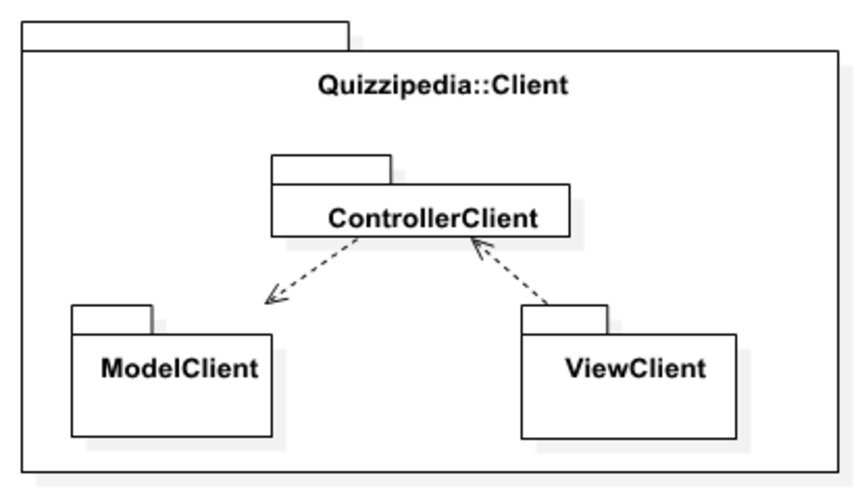
\includegraphics[width=\textwidth]{ImgST/quizzipedia-client.pdf}}
\caption{Schema Componente Quizzipedia::Client}
\end{figure}
\subsection{Quizzipedia::Client::ModelClient}
Rappresenta il modello dei dati che verranno utilizzati dal sistema lato client.
\begin{figure}[H]
\centering
\noindent\makebox[\textwidth]{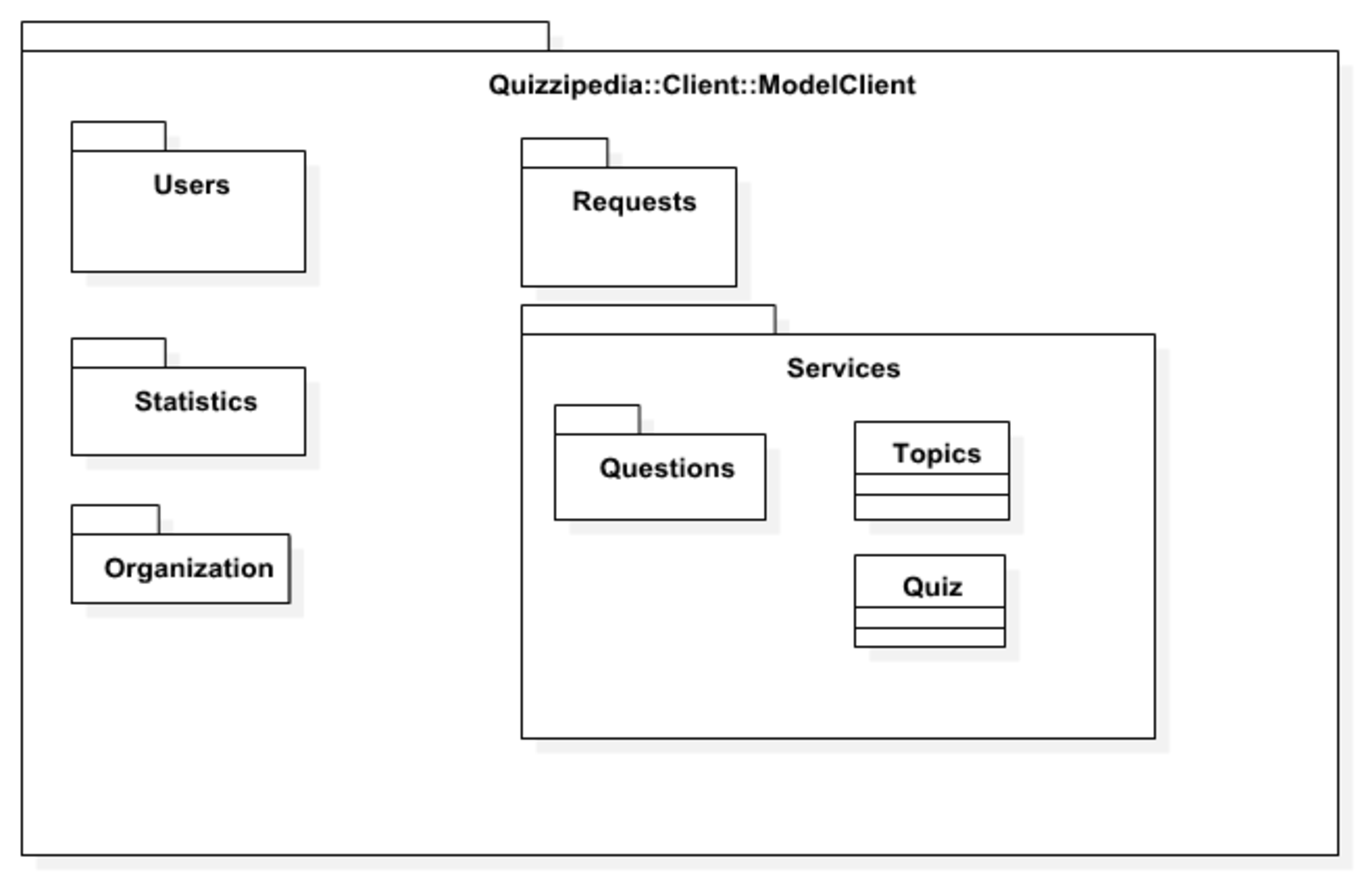
\includegraphics[width=\textwidth]{ImgST/quizzipedia-client-modelclient.pdf}}
\caption{Schema Componente Quizzipedia::Client::ModelClient}
\end{figure}
\subsubsection{Componenti contenute}
\begin{itemize}
\item Quizzipedia::Client::ModelClient::Organization
\item Quizzipedia::Client::ModelClient::Requests
\item Quizzipedia::Client::ModelClient::Services
\item Quizzipedia::Client::ModelClient::Statistics
\item Quizzipedia::Client::ModelClient::Users
\end{itemize}
\subsection{Quizzipedia::Client::ModelClient::Organization}
La componente gestisce le classi e gli enti, ovvero il sistema in base a cui sono organizzati gli utenti nel sistema.
\begin{figure}[H]
\centering
\noindent\makebox[\textwidth]{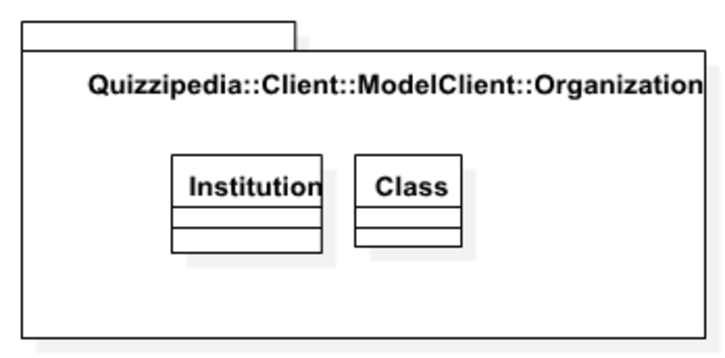
\includegraphics[width=\textwidth]{ImgST/quizzipedia-client-modelclient-organization.pdf}}
\caption{Schema Componente Quizzipedia::Client::ModelClient::Organization}
\end{figure}
\subsubsection{Classe Class}
Contiene informazioni relative alla struttura delle classi.
\begin{figure}[H]
\centering
\noindent\makebox[\textwidth]{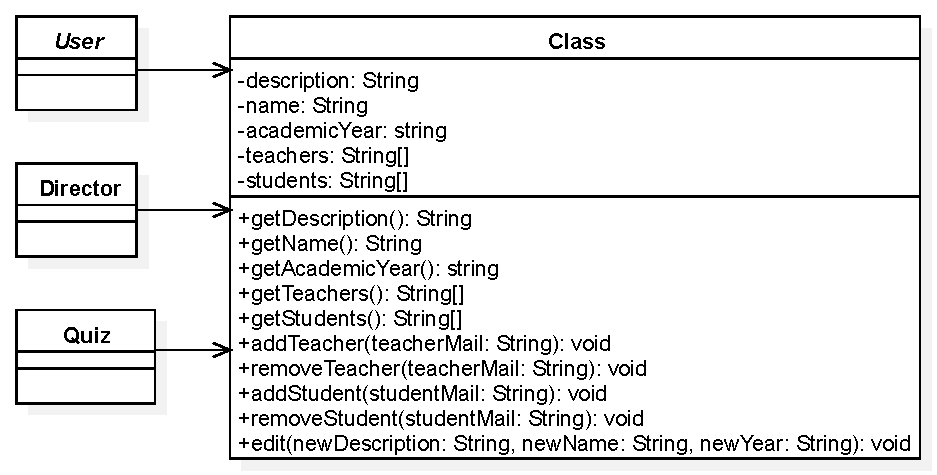
\includegraphics[width=\textwidth]{ImgST/quizzipedia-client-modelclient-organization-class.pdf}}
\caption{Schema Classe Quizzipedia::Client::ModelClient::Organization::Class}
\end{figure}
\myparagraph{Relazioni con altre classi}
\begin{itemize}
\item Quizzipedia::Client::ModelClient::Organization::Institution
\end{itemize}
\subsubsection{Classe Institution}
La classe contiene le informazioni relative alla struttura dell'ente.
\begin{figure}[H]
\centering
\noindent\makebox[\textwidth]{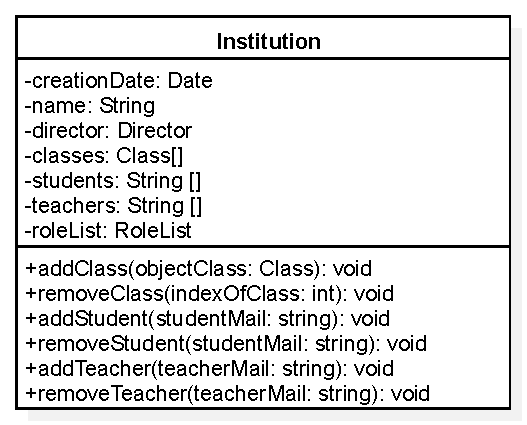
\includegraphics[width=\textwidth]{ImgST/quizzipedia-client-modelclient-organization-institution.pdf}}
\caption{Schema Classe Quizzipedia::Client::ModelClient::Organization::Institution}
\end{figure}
\subsection{Quizzipedia::Client::ModelClient::Requests}
Questo package contiene le classi necessarie a gestire le richieste di ruolo e di classe degli utenti.
\begin{figure}[H]
\centering
\noindent\makebox[\textwidth]{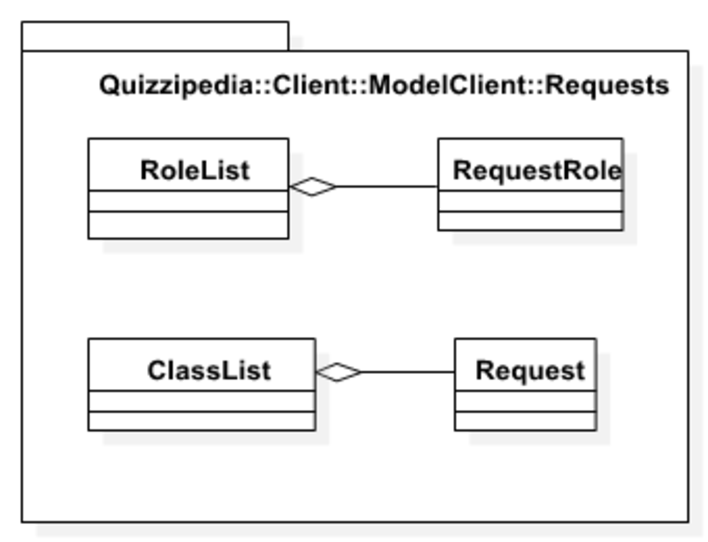
\includegraphics[width=\textwidth]{ImgST/quizzipedia-client-modelclient-requests.pdf}}
\caption{Schema Componente Quizzipedia::Client::ModelClient::Requests}
\end{figure}
\subsubsection{Classe ClassList}
Questa classe gestisce le richieste da parte di Docenti o Studenti per l'assegnazione a una specifica classe.
\begin{figure}[H]
\centering
\noindent\makebox[\textwidth]{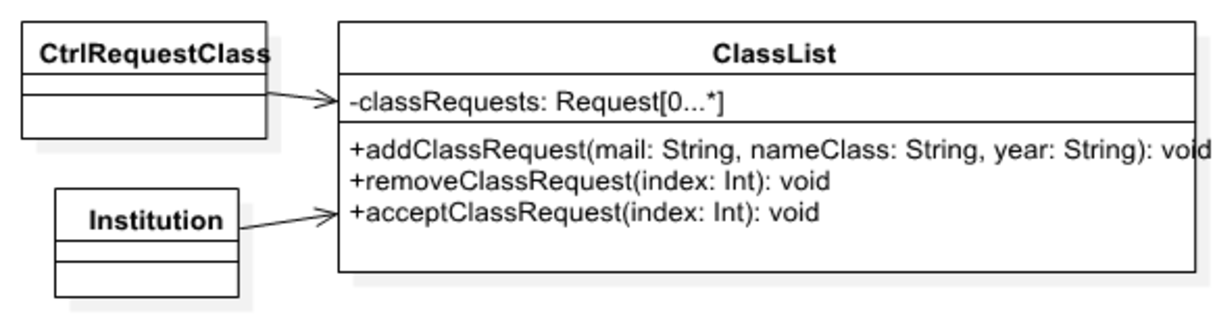
\includegraphics[width=\textwidth]{ImgST/quizzipedia-client-modelclient-requests-classlist.pdf}}
\caption{Schema Classe Quizzipedia::Client::ModelClient::Requests::ClassList}
\end{figure}
\myparagraph{Relazioni con altre classi}
\begin{itemize}
\item Quizzipedia::Client::ModelClient::Requests::Request
\end{itemize}
\subsubsection{Classe Request}
La classe memorizza l'utente che invia la richiesta di inserimento in una classe e la classe per cui ha fatto richiesta.
\begin{figure}[H]
\centering
\noindent\makebox[\textwidth]{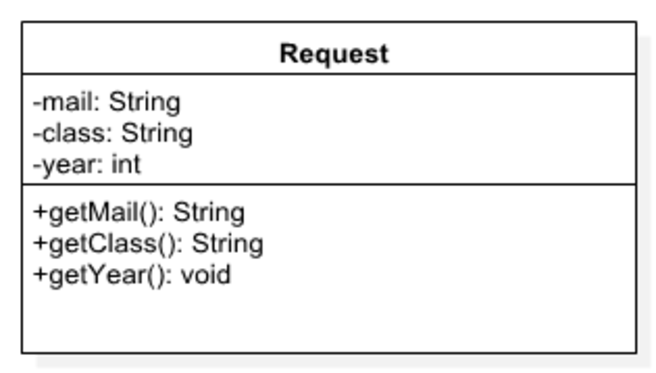
\includegraphics[width=\textwidth]{ImgST/quizzipedia-client-modelclient-requests-request.pdf}}
\caption{Schema Classe Quizzipedia::Client::ModelClient::Requests::Request}
\end{figure}
\subsubsection{Classe RolesList}
Gli utenti senza ruolo inviano le proprie richieste per l'assegnazione al ruolo di studente o docente al Responsabile di un Ente. Questa classe gestisce tali richieste.
\begin{figure}[H]
\centering
\noindent\makebox[\textwidth]{\includegraphics[width=\textwidth]{ImgST/quizzipedia-client-modelclient-requests-roleslist.pdf}}
\caption{Schema Classe Quizzipedia::Client::ModelClient::Requests::RolesList}
\end{figure}
\subsection{Quizzipedia::Client::ModelClient::Services}
Il package racchiude i modelli necessari alla creazione di domande e quiz, i servizi principali offerti dal nostro prodotto.
\begin{figure}[H]
\centering
\noindent\makebox[\textwidth]{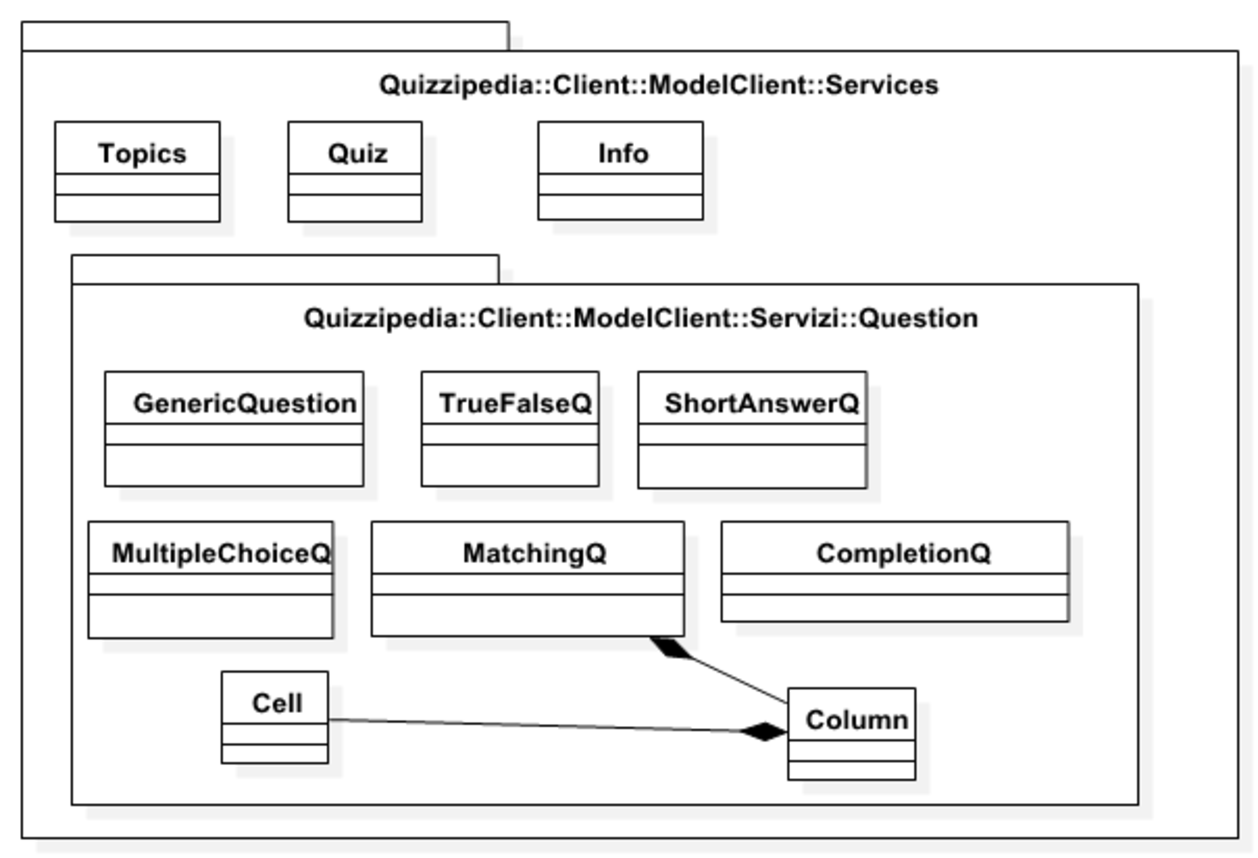
\includegraphics[width=\textwidth]{ImgST/quizzipedia-client-modelclient-services.pdf}}
\caption{Schema Componente Quizzipedia::Client::ModelClient::Services}
\end{figure}
\subsubsection{Componenti contenute}
\begin{itemize}
\item Quizzipedia::Client::ModelClient::Services::Questions
\end{itemize}
\subsubsection{Classe Info}
Riassume le informazioni principali su quiz e domande, necessarie per una presentazione sintetica e puntuale all'utente. È poi possibile risalire alla domanda o al quiz completi.
\begin{figure}[H]
\centering
\noindent\makebox[\textwidth]{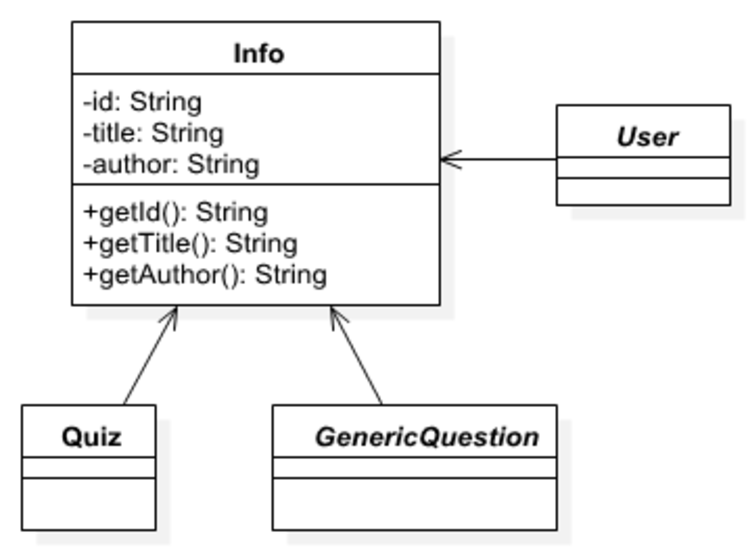
\includegraphics[width=\textwidth]{ImgST/quizzipedia-client-modelclient-services-info.pdf}}
\caption{Schema Classe Quizzipedia::Client::ModelClient::Services::Info}
\end{figure}
\subsubsection{Classe Quiz}
Include la struttura del quiz.
\begin{figure}[H]
\centering
\noindent\makebox[\textwidth]{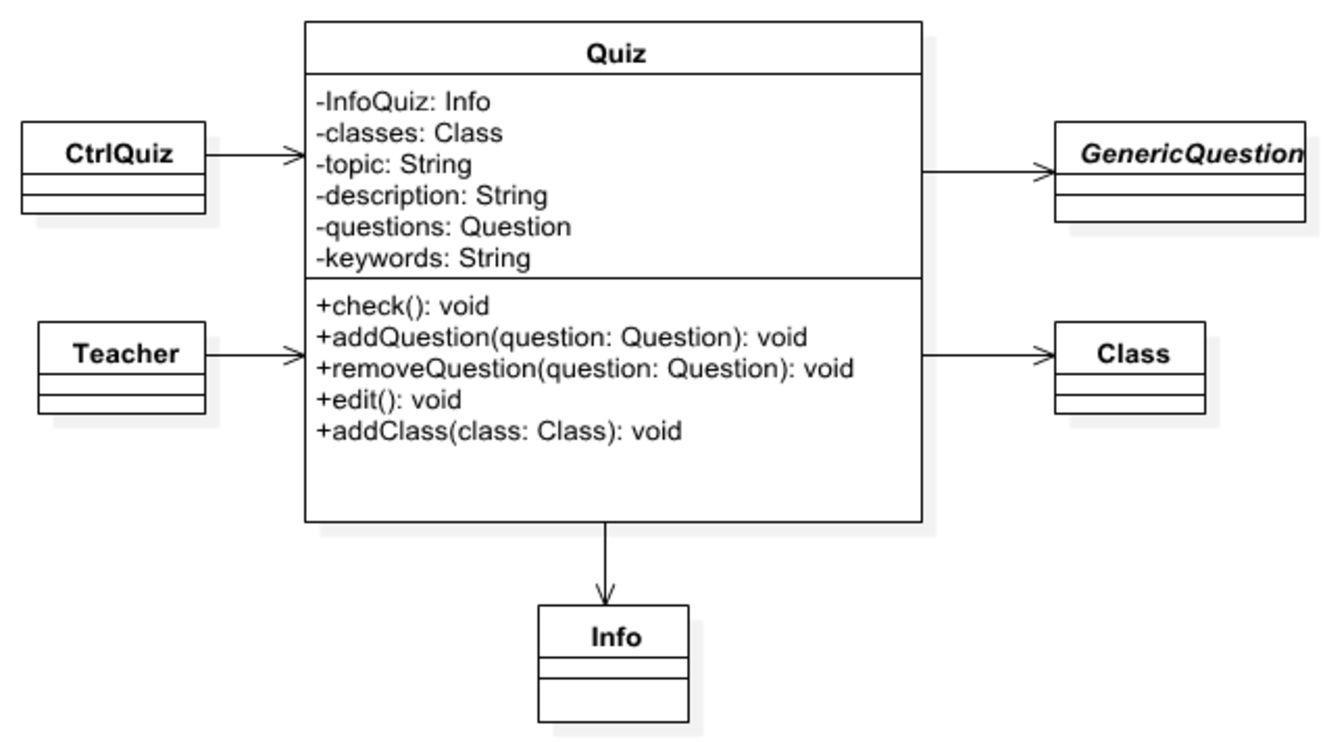
\includegraphics[width=\textwidth]{ImgST/quizzipedia-client-modelclient-services-quiz.pdf}}
\caption{Schema Classe Quizzipedia::Client::ModelClient::Services::Quiz}
\end{figure}
\myparagraph{Relazioni con altre classi}
\begin{itemize}
\item Quizzipedia::Client::ModelClient::Services::Topics
\end{itemize}
\subsubsection{Classe Topics}
Modella la struttura necessaria a memorizzare la lista di argomenti. A ogni domanda e a ogni quiz verranno poi associati i relativi argomenti .
\begin{figure}[H]
\centering
\noindent\makebox[\textwidth]{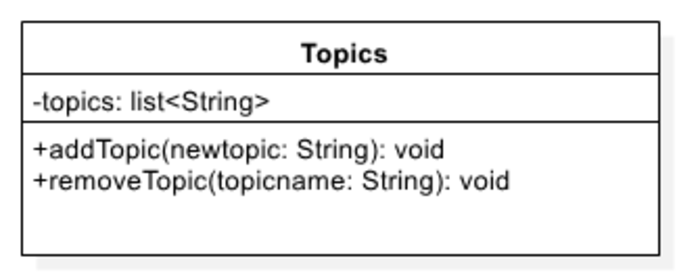
\includegraphics[width=\textwidth]{ImgST/quizzipedia-client-modelclient-services-topics.pdf}}
\caption{Schema Classe Quizzipedia::Client::ModelClient::Services::Topics}
\end{figure}
\subsection{Quizzipedia::Client::ModelClient::Services::Questions}
Descrive il modo in cui sono strutturati i vari tipi di domande che l'utente può incontrare durante la creazione o la compilazione di quiz.
\begin{figure}[H]
\centering
\noindent\makebox[\textwidth]{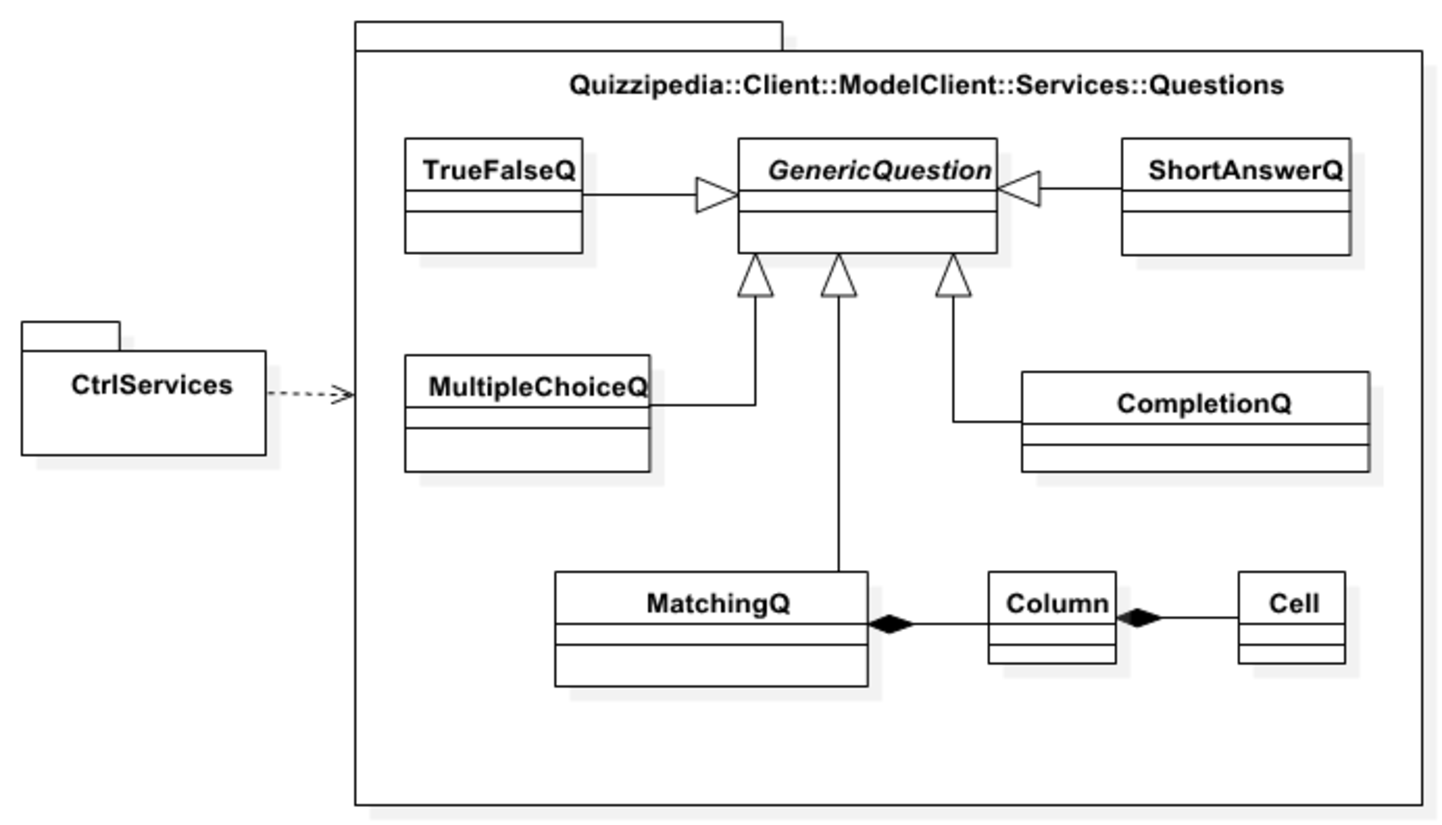
\includegraphics[width=\textwidth]{ImgST/quizzipedia-client-modelclient-services-questions.pdf}}
\caption{Schema Componente Quizzipedia::Client::ModelClient::Services::Questions}
\end{figure}
\subsubsection{Classe Cell}
La classe descrive ogni singola riga (quindi ogni opzione) della colonna della domanda a collegamento.
\begin{figure}[H]
\centering
\noindent\makebox[\textwidth]{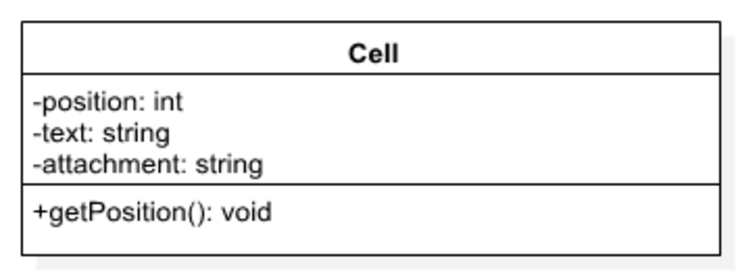
\includegraphics[width=\textwidth]{ImgST/quizzipedia-client-modelclient-services-questions-cell.pdf}}
\caption{Schema Classe Quizzipedia::Client::ModelClient::Services::Questions::Cell}
\end{figure}
\subsubsection{Classe Column}
La classe descrive le colonne della domanda a collegamenti.
\begin{figure}[H]
\centering
\noindent\makebox[\textwidth]{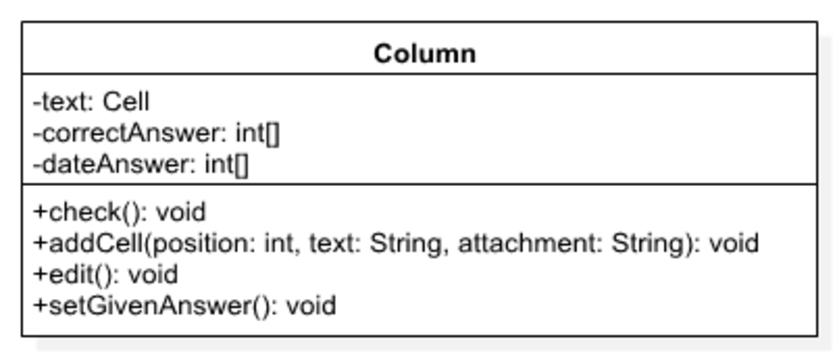
\includegraphics[width=\textwidth]{ImgST/quizzipedia-client-modelclient-services-questions-column.pdf}}
\caption{Schema Classe Quizzipedia::Client::ModelClient::Services::Questions::Column}
\end{figure}
\myparagraph{Relazioni con altre classi}
\begin{itemize}
\item Quizzipedia::Client::ModelClient::Services::Questions::Cell
\end{itemize}
\subsubsection{Classe CompletionQ}
Descrive le domande a completamento. Il docente fornirà un testo incompleto e una lista di possibili completamenti; lo studente dovrà inserire le parole adeguate nella giusta posizione.
\begin{figure}[H]
\centering
\noindent\makebox[\textwidth]{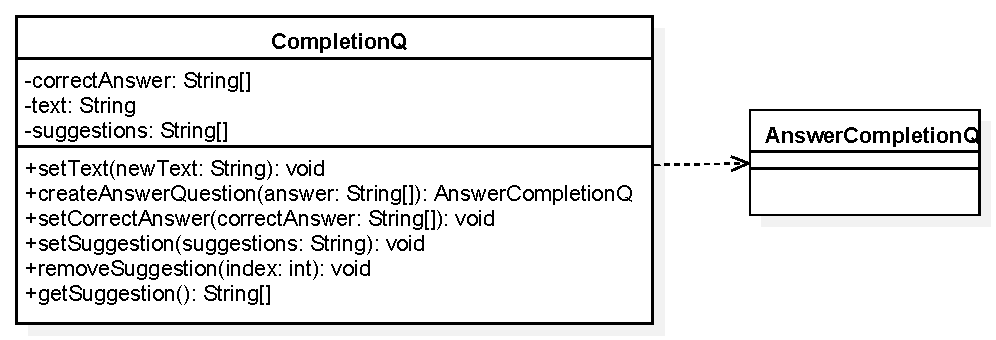
\includegraphics[width=\textwidth]{ImgST/quizzipedia-client-modelclient-services-questions-completionq.pdf}}
\caption{Schema Classe Quizzipedia::Client::ModelClient::Services::Questions::CompletionQ}
\end{figure}
\subsubsection{Classe GenericQuestion}
Descrive le parti comuni a tutti i tipi di domanda presenti nel sistema.
\begin{figure}[H]
\centering
\noindent\makebox[\textwidth]{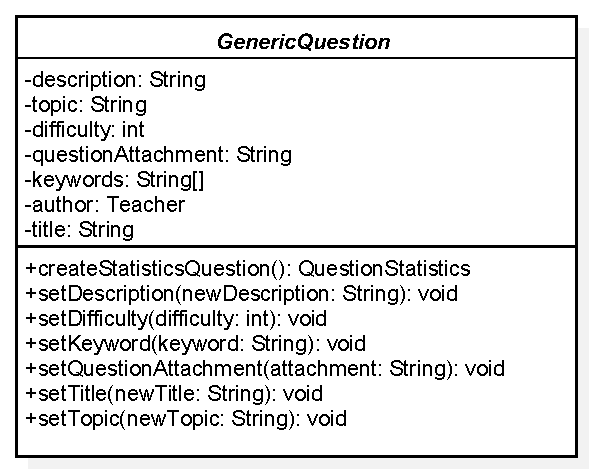
\includegraphics[width=\textwidth]{ImgST/quizzipedia-client-modelclient-services-questions-genericquestion.pdf}}
\caption{Schema Classe Quizzipedia::Client::ModelClient::Services::Questions::GenericQuestion}
\end{figure}
\myparagraph{Relazioni con altre classi}
\begin{itemize}
\item Quizzipedia::Client::ModelClient::Services::Questions::CompletionQ
\item Quizzipedia::Client::ModelClient::Services::Questions::MatchingQ
\item Quizzipedia::Client::ModelClient::Services::Questions::MultipleChoiceQ
\item Quizzipedia::Client::ModelClient::Services::Questions::ShortAnswerQ
\item Quizzipedia::Client::ModelClient::Services::Questions::TrueFalseQ
\item Quizzipedia::Client::ModelClient::Services::Topics
\end{itemize}
\subsubsection{Classe MatchingQ}
La struttura descrive le domande a collegamento. L'utente dovrà formare la risposa collegando entrate da un numero variabile di colonne .
\begin{figure}[H]
\centering
\noindent\makebox[\textwidth]{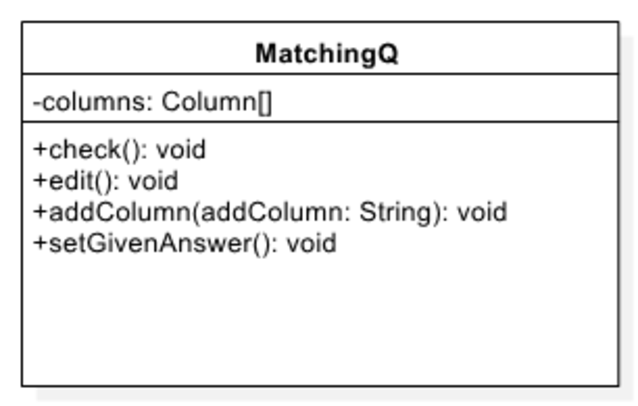
\includegraphics[width=\textwidth]{ImgST/quizzipedia-client-modelclient-services-questions-matchingq.pdf}}
\caption{Schema Classe Quizzipedia::Client::ModelClient::Services::Questions::MatchingQ}
\end{figure}
\myparagraph{Relazioni con altre classi}
\begin{itemize}
\item Quizzipedia::Client::ModelClient::Services::Questions::Column
\end{itemize}
\subsubsection{Classe MultipleChoiceQ}
La struttura descrive le domande a scelta multipla; viene presentata una lista di opzioni tra cui scegliere quelle corrette.
\begin{figure}[H]
\centering
\noindent\makebox[\textwidth]{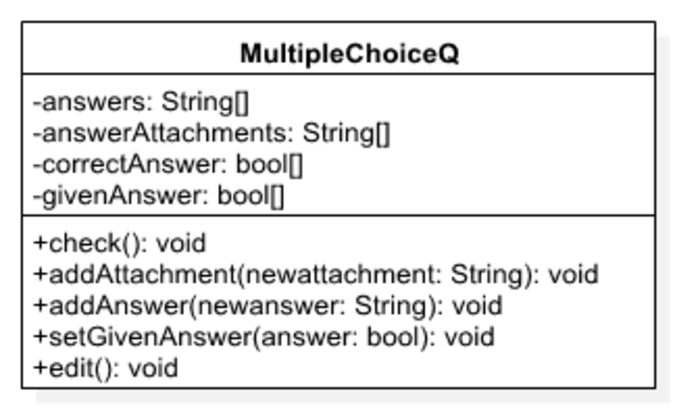
\includegraphics[width=\textwidth]{ImgST/quizzipedia-client-modelclient-services-questions-multiplechoiceq.pdf}}
\caption{Schema Classe Quizzipedia::Client::ModelClient::Services::Questions::MultipleChoiceQ}
\end{figure}
\subsubsection{Classe ShortAnswerQ}
La struttura descrive le domande aperte, ovvero quelle la cui risposta consiste in un termine o una frase specifici.
\begin{figure}[H]
\centering
\noindent\makebox[\textwidth]{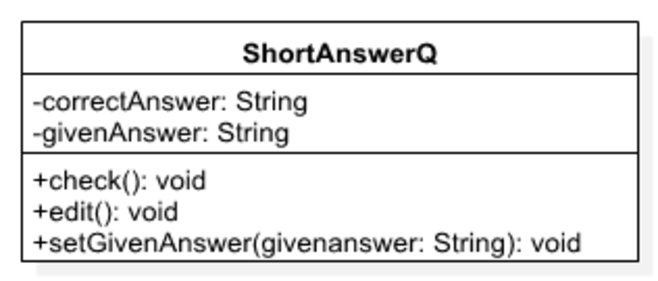
\includegraphics[width=\textwidth]{ImgST/quizzipedia-client-modelclient-services-questions-shortanswerq.pdf}}
\caption{Schema Classe Quizzipedia::Client::ModelClient::Services::Questions::ShortAnswerQ}
\end{figure}
\subsubsection{Classe TrueFalseQ}
Viene descritta la struttura delle domande che prevedono di decidere la veridicità di un'affermazione.
\begin{figure}[H]
\centering
\noindent\makebox[\textwidth]{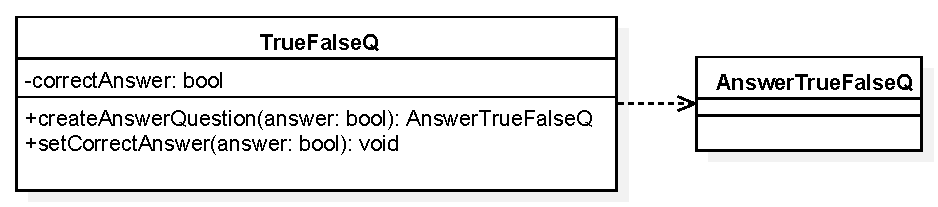
\includegraphics[width=\textwidth]{ImgST/quizzipedia-client-modelclient-services-questions-truefalseq.pdf}}
\caption{Schema Classe Quizzipedia::Client::ModelClient::Services::Questions::TrueFalseQ}
\end{figure}
\subsection{Quizzipedia::Client::ModelClient::Statistics}
Qui sono raccolte le classi con il compito di reperire informazioni sulle statistiche dal server e presentarle al'utente finale. Sono disponibili statistiche per le domande, per i quiz e per gli studenti di ogni classe.
\begin{figure}[H]
\centering
\noindent\makebox[\textwidth]{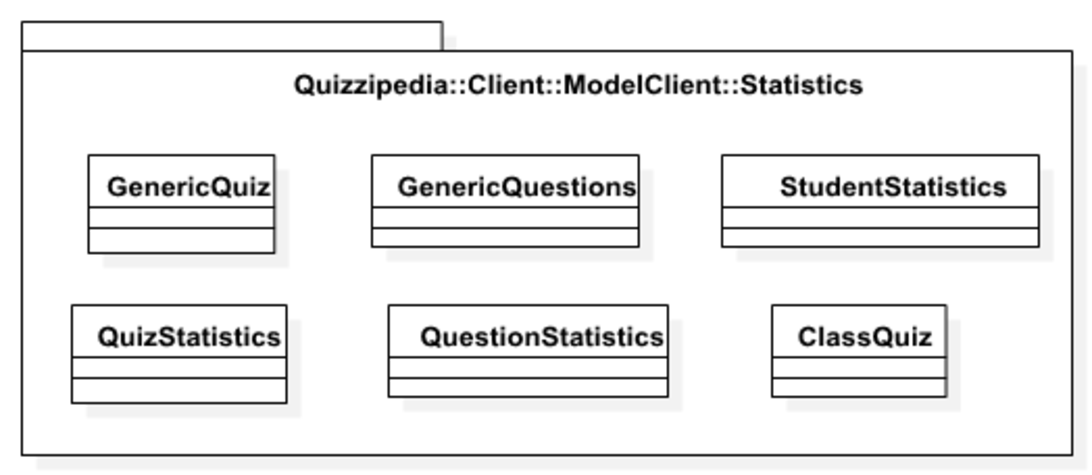
\includegraphics[width=\textwidth]{ImgST/quizzipedia-client-modelclient-statistics.pdf}}
\caption{Schema Componente Quizzipedia::Client::ModelClient::Statistics}
\end{figure}
\subsubsection{Classe ClassQuiz}
La classe raccoglie le statistiche riguardanti gli studenti di una classe relativamente a un quiz assegnato.
\begin{figure}[H]
\centering
\noindent\makebox[\textwidth]{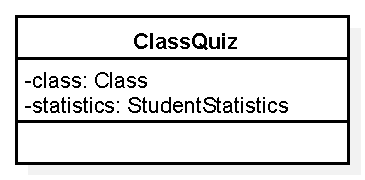
\includegraphics[width=\textwidth]{ImgST/quizzipedia-client-modelclient-statistics-classquiz.pdf}}
\caption{Schema Classe Quizzipedia::Client::ModelClient::Statistics::ClassQuiz}
\end{figure}
\myparagraph{Relazioni con altre classi}
\begin{itemize}
\item Quizzipedia::Client::ModelClient::Statistics::StudentStatistics
\end{itemize}
\subsubsection{Classe QuestionGenerics}
Le statistiche relative a più domande vengono raccolte e organizzate per permetterne la visualizzazione agli utenti.
\begin{figure}[H]
\centering
\noindent\makebox[\textwidth]{\includegraphics[width=\textwidth]{ImgST/quizzipedia-client-modelclient-statistics-questiongenerics.pdf}}
\caption{Schema Classe Quizzipedia::Client::ModelClient::Statistics::QuestionGenerics}
\end{figure}
\myparagraph{Relazioni con altre classi}
\begin{itemize}
\item Quizzipedia::Client::ModelClient::Statistics::QuestionStatistics
\end{itemize}
\subsubsection{Classe QuestionStatistics}
La classe raccoglie le statistiche principali riguardanti una singola domanda. Da qui è poi possibile risalire alla domanda.
\begin{figure}[H]
\centering
\noindent\makebox[\textwidth]{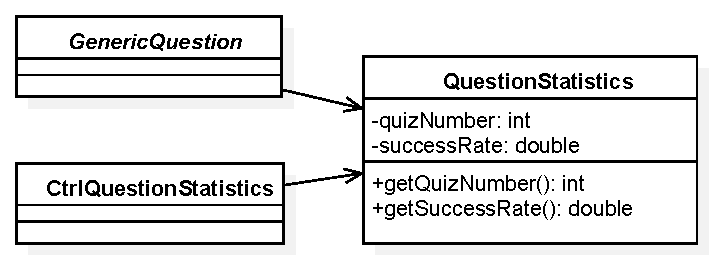
\includegraphics[width=\textwidth]{ImgST/quizzipedia-client-modelclient-statistics-questionstatistics.pdf}}
\caption{Schema Classe Quizzipedia::Client::ModelClient::Statistics::QuestionStatistics}
\end{figure}
\subsubsection{Classe QuizGenerics}
Le statistiche relative a più quiz vengono raccolte e organizzate per permetterne la visualizzazione agli utenti.
\begin{figure}[H]
\centering
\noindent\makebox[\textwidth]{\includegraphics[width=\textwidth]{ImgST/quizzipedia-client-modelclient-statistics-quizgenerics.pdf}}
\caption{Schema Classe Quizzipedia::Client::ModelClient::Statistics::QuizGenerics}
\end{figure}
\myparagraph{Relazioni con altre classi}
\begin{itemize}
\item Quizzipedia::Client::ModelClient::Statistics::QuizStatistics
\end{itemize}
\subsubsection{Classe QuizStatistics}
La classe raccoglie le statistiche principali riguardanti un singolo quiz. Da qui è poi possibile ottenere il quiz in questione.
\begin{figure}[H]
\centering
\noindent\makebox[\textwidth]{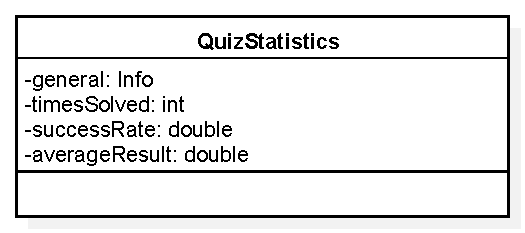
\includegraphics[width=\textwidth]{ImgST/quizzipedia-client-modelclient-statistics-quizstatistics.pdf}}
\caption{Schema Classe Quizzipedia::Client::ModelClient::Statistics::QuizStatistics}
\end{figure}
\subsubsection{Classe StudentStatistics}
Qui è memorizzata la struttura che permette di associare a un utente le statistiche riguardanti un quiz (voto, superamento).
\begin{figure}[H]
\centering
\noindent\makebox[\textwidth]{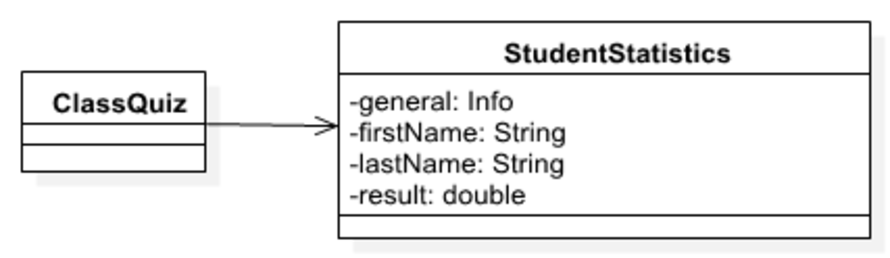
\includegraphics[width=\textwidth]{ImgST/quizzipedia-client-modelclient-statistics-studentstatistics.pdf}}
\caption{Schema Classe Quizzipedia::Client::ModelClient::Statistics::StudentStatistics}
\end{figure}
\subsection{Quizzipedia::Client::ModelClient::Users}
Raccoglie le classi necessarie a descrivere le diverse tipologie di utente che possono accedere al sistema.
\begin{figure}[H]
\centering
\noindent\makebox[\textwidth]{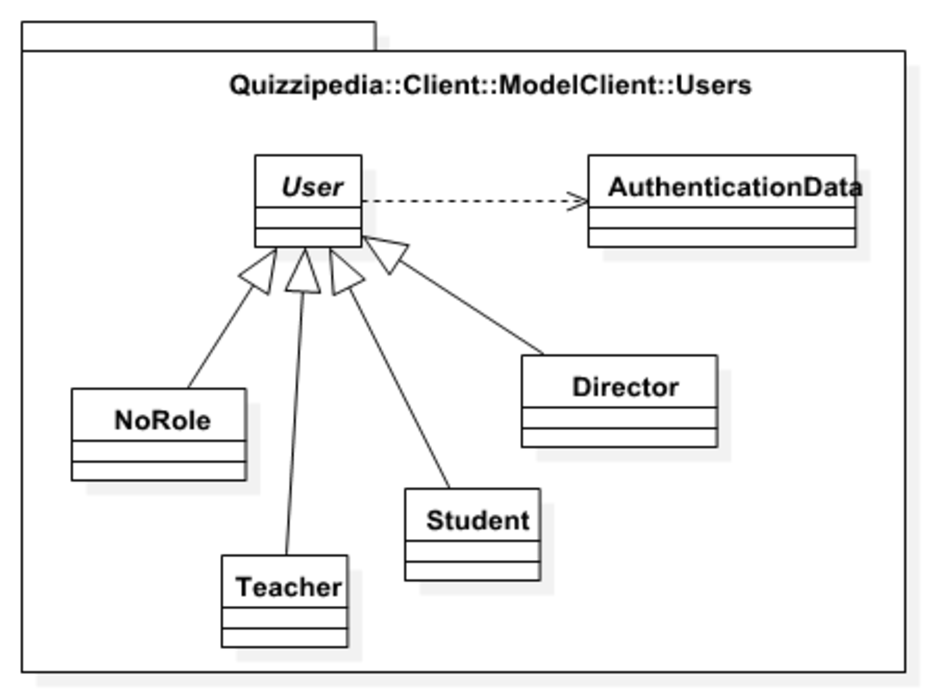
\includegraphics[width=\textwidth]{ImgST/quizzipedia-client-modelclient-users.pdf}}
\caption{Schema Componente Quizzipedia::Client::ModelClient::Users}
\end{figure}
\subsubsection{Classe AutheniticationData}
Questa classe gestisce le informazioni di autenticazione comuni a tutti gli utenti.
\begin{figure}[H]
\centering
\noindent\makebox[\textwidth]{\includegraphics[width=\textwidth]{ImgST/quizzipedia-client-modelclient-users-autheniticationdata.pdf}}
\caption{Schema Classe Quizzipedia::Client::ModelClient::Users::AutheniticationData}
\end{figure}
\myparagraph{Relazioni con altre classi}
\begin{itemize}
\item Quizzipedia::Client::ModelClient::Users::User
\end{itemize}
\subsubsection{Classe Director}
Rappresenta un Responsabile, ovvero colui che gestisce Docenti e Studenti per ogni Ente del sistema.
\begin{figure}[H]
\centering
\noindent\makebox[\textwidth]{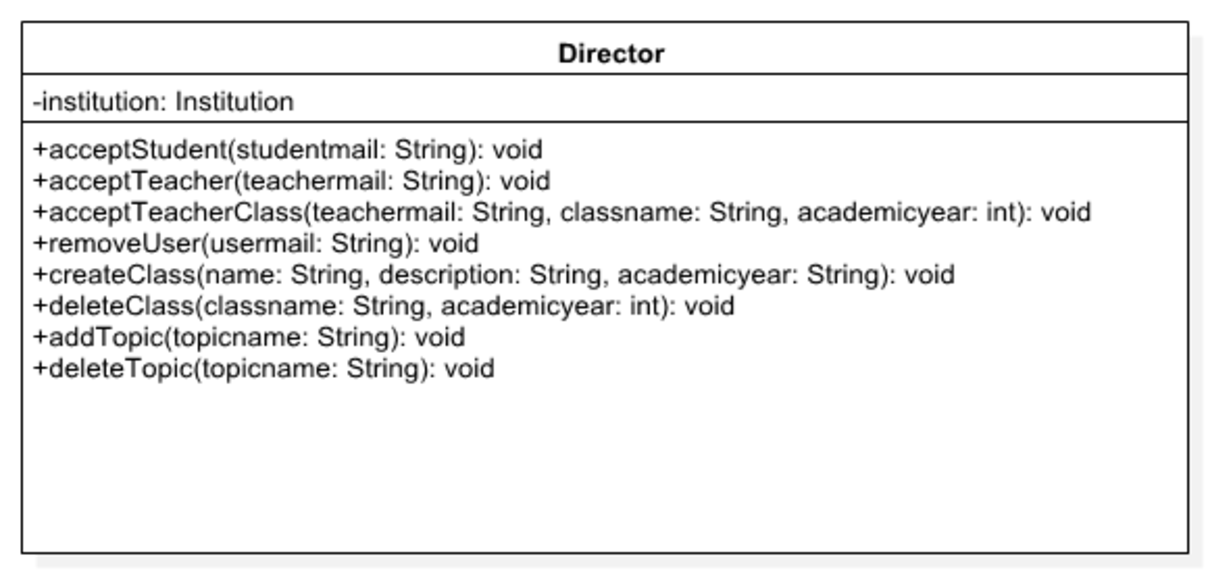
\includegraphics[width=\textwidth]{ImgST/quizzipedia-client-modelclient-users-director.pdf}}
\caption{Schema Classe Quizzipedia::Client::ModelClient::Users::Director}
\end{figure}
\subsubsection{Classe NoRole}
Rappresenta gli utenti senza ruolo del sistema; ovvero coloro che si sono registrati e autenticati ma non hanno ancora fatto richiesta per l'assegnazione ad alcun ruolo.
\begin{figure}[H]
\centering
\noindent\makebox[\textwidth]{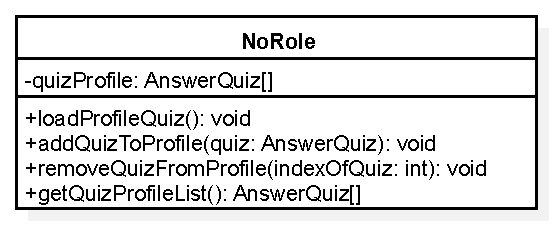
\includegraphics[width=\textwidth]{ImgST/quizzipedia-client-modelclient-users-norole.pdf}}
\caption{Schema Classe Quizzipedia::Client::ModelClient::Users::NoRole}
\end{figure}
\subsubsection{Classe Student}
Rappresenta uno studente del sistema e implementa le sue funzioni specifiche oltre a quelle ereditate da Utente.
\begin{figure}[H]
\centering
\noindent\makebox[\textwidth]{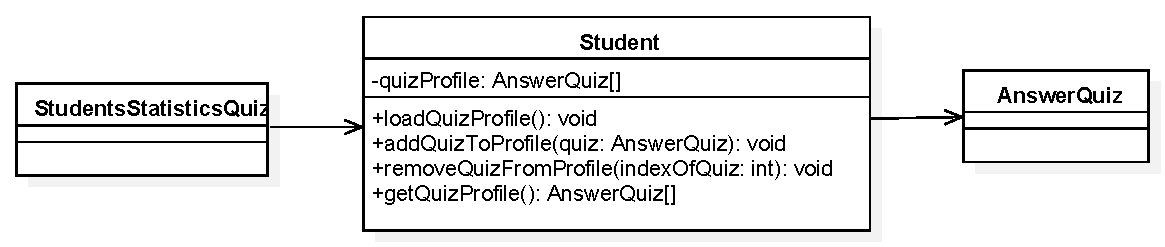
\includegraphics[width=\textwidth]{ImgST/quizzipedia-client-modelclient-users-student.pdf}}
\caption{Schema Classe Quizzipedia::Client::ModelClient::Users::Student}
\end{figure}
\subsubsection{Classe Teacher}
Rappresenta un docente del sistema e ne implementa le funzionalità specifiche in aggiunta a quelle comuni a tutti gli utenti.
\begin{figure}[H]
\centering
\noindent\makebox[\textwidth]{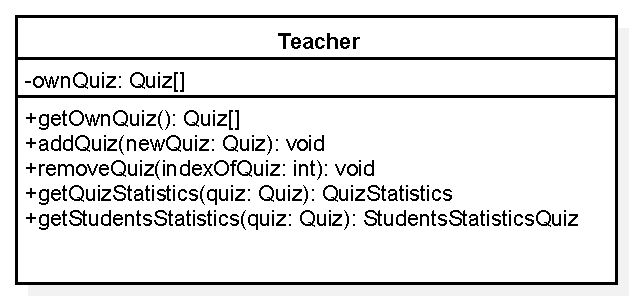
\includegraphics[width=\textwidth]{ImgST/quizzipedia-client-modelclient-users-teacher.pdf}}
\caption{Schema Classe Quizzipedia::Client::ModelClient::Users::Teacher}
\end{figure}
\subsubsection{Classe User}
Questa è una classe astratta e raccoglie le funzionalità comuni a tutti gli utenti.
\begin{figure}[H]
\centering
\noindent\makebox[\textwidth]{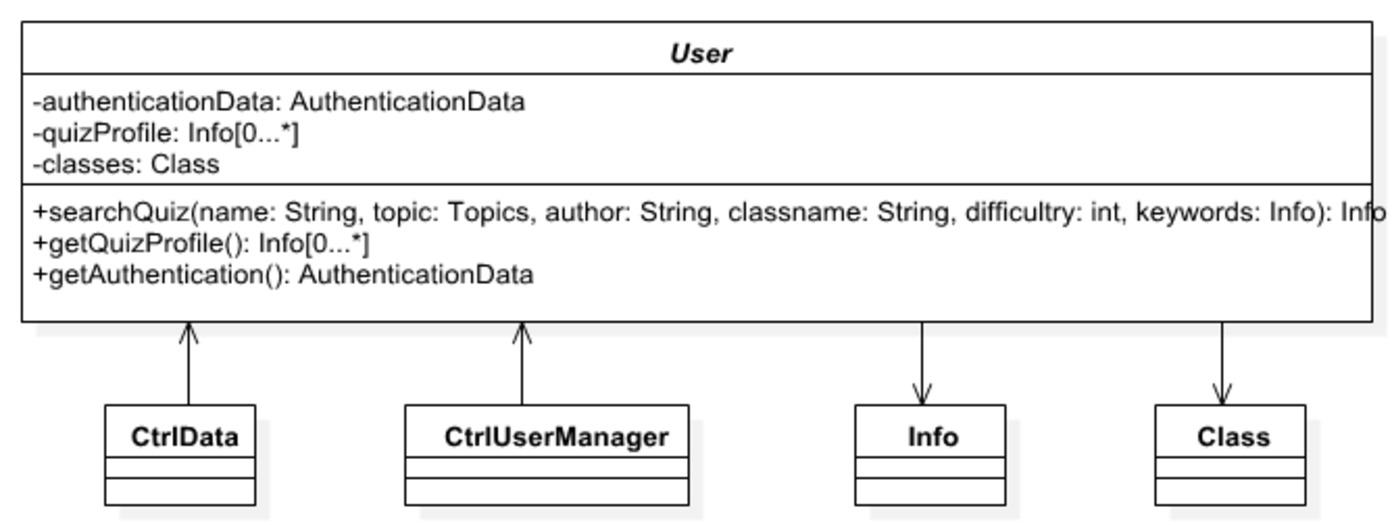
\includegraphics[width=\textwidth]{ImgST/quizzipedia-client-modelclient-users-user.pdf}}
\caption{Schema Classe Quizzipedia::Client::ModelClient::Users::User}
\end{figure}
\myparagraph{Relazioni con altre classi}
\begin{itemize}
\item Quizzipedia::Client::ModelClient::Users::Director
\item Quizzipedia::Client::ModelClient::Users::NoRole
\item Quizzipedia::Client::ModelClient::Users::Student
\item Quizzipedia::Client::ModelClient::Users::Teacher
\end{itemize}
\subsection{Quizzipedia::Client::ViewClient}
Racchiude tutte le componenti necessarie per presentare il prodotto all'utente.
\begin{figure}[H]
\centering
\noindent\makebox[\textwidth]{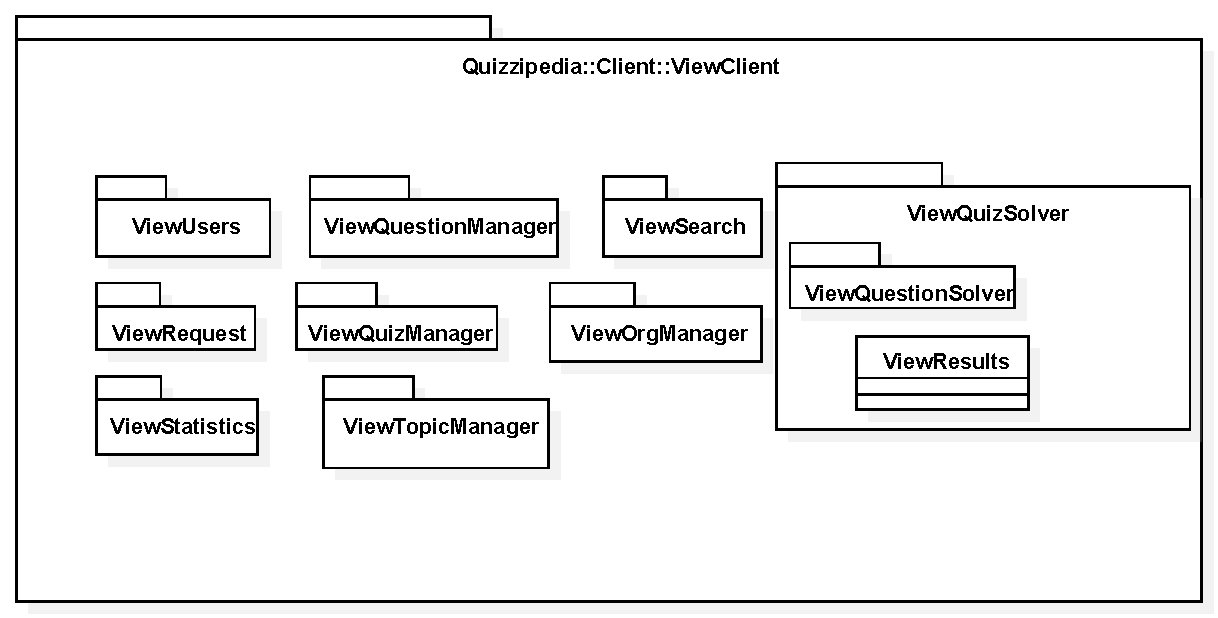
\includegraphics[width=\textwidth]{ImgST/quizzipedia-client-viewclient.pdf}}
\caption{Schema Componente Quizzipedia::Client::ViewClient}
\end{figure}
\subsubsection{Componenti contenute}
\begin{itemize}
\item Quizzipedia::Client::ViewClient::ViewErrors
\item Quizzipedia::Client::ViewClient::ViewOrgManager
\item Quizzipedia::Client::ViewClient::ViewQuestionManager
\item Quizzipedia::Client::ViewClient::ViewQuizManager
\item Quizzipedia::Client::ViewClient::ViewQuizSolver
\item Quizzipedia::Client::ViewClient::ViewRequests
\item Quizzipedia::Client::ViewClient::ViewSearch
\item Quizzipedia::Client::ViewClient::ViewStatistics
\item Quizzipedia::Client::ViewClient::ViewTopicManager
\item Quizzipedia::Client::ViewClient::ViewUsers
\end{itemize}
\subsection{Quizzipedia::Client::ViewClient::ViewErrors}
Il package raccoglie tutte le finestre di errore che il sistema può, eventualmente, visualizzare.
\begin{figure}[H]
\centering
\noindent\makebox[\textwidth]{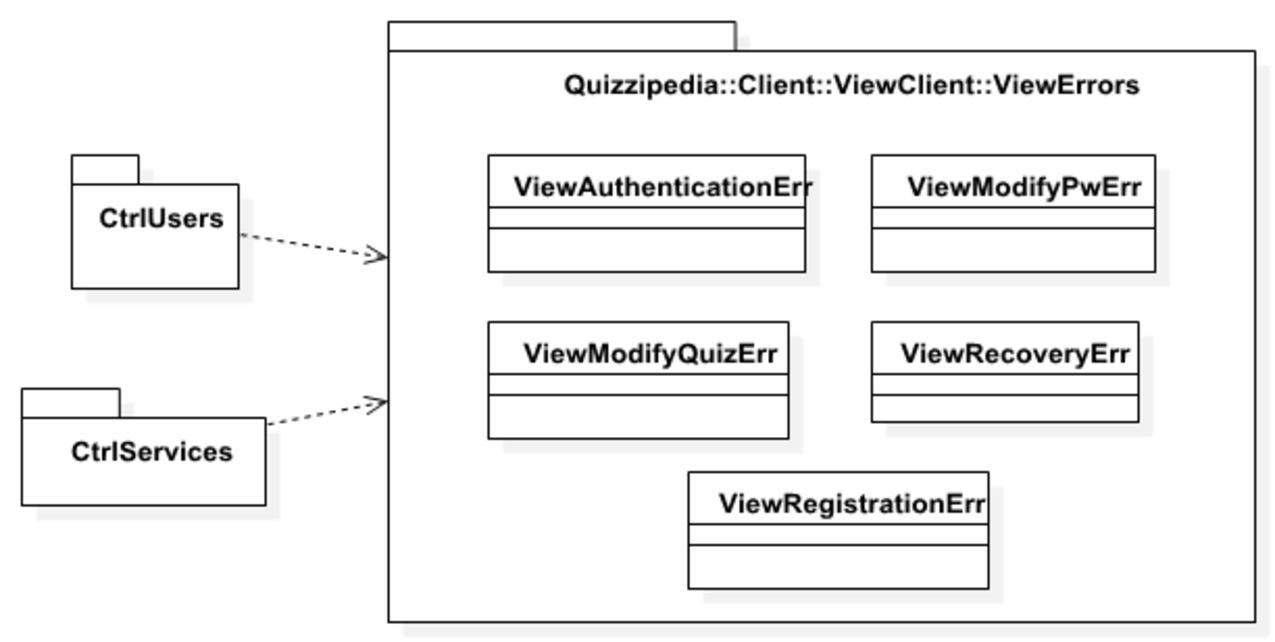
\includegraphics[width=\textwidth]{ImgST/quizzipedia-client-viewclient-viewerrors.pdf}}
\caption{Schema Componente Quizzipedia::Client::ViewClient::ViewErrors}
\end{figure}
\subsubsection{Classe ViewAuthenticationErr}
La classe si occupa della visualizzazione del messaggio di errore in fase di autenticazione.
\begin{figure}[H]
\centering
\noindent\makebox[\textwidth]{\includegraphics[width=\textwidth]{ImgST/quizzipedia-client-viewclient-viewerrors-viewauthenticationerr.pdf}}
\caption{Schema Classe Quizzipedia::Client::ViewClient::ViewErrors::ViewAuthenticationErr}
\end{figure}
\subsubsection{Classe ViewModifyPwErr}
La classe si occupa della visualizzazione del messaggio di errore in fase modifica della password.
\begin{figure}[H]
\centering
\noindent\makebox[\textwidth]{\includegraphics[width=\textwidth]{ImgST/quizzipedia-client-viewclient-viewerrors-viewmodifypwerr.pdf}}
\caption{Schema Classe Quizzipedia::Client::ViewClient::ViewErrors::ViewModifyPwErr}
\end{figure}
\subsubsection{Classe ViewModifyQuizErr}
La classe si occupa della visualizzazione del messaggio di errore in fase di modifica di un quiz.
\begin{figure}[H]
\centering
\noindent\makebox[\textwidth]{\includegraphics[width=\textwidth]{ImgST/quizzipedia-client-viewclient-viewerrors-viewmodifyquizerr.pdf}}
\caption{Schema Classe Quizzipedia::Client::ViewClient::ViewErrors::ViewModifyQuizErr}
\end{figure}
\subsubsection{Classe ViewRecoveryErr}
La classe si occupa della visualizzazione del messaggio di errore in fase di recupero password.
\begin{figure}[H]
\centering
\noindent\makebox[\textwidth]{\includegraphics[width=\textwidth]{ImgST/quizzipedia-client-viewclient-viewerrors-viewrecoveryerr.pdf}}
\caption{Schema Classe Quizzipedia::Client::ViewClient::ViewErrors::ViewRecoveryErr}
\end{figure}
\subsubsection{Classe ViewRegistrationErr}
La classe si occupa della visualizzazione del messaggio di errore in fase di registrazione.
\begin{figure}[H]
\centering
\noindent\makebox[\textwidth]{\includegraphics[width=\textwidth]{ImgST/quizzipedia-client-viewclient-viewerrors-viewregistrationerr.pdf}}
\caption{Schema Classe Quizzipedia::Client::ViewClient::ViewErrors::ViewRegistrationErr}
\end{figure}
\subsection{Quizzipedia::Client::ViewClient::ViewOrgManager}
Qui sono raccolte le classi responsabili della presentazione delle pagine da cui sarà possibile gestire le classi e gli enti.
\begin{figure}[H]
\centering
\noindent\makebox[\textwidth]{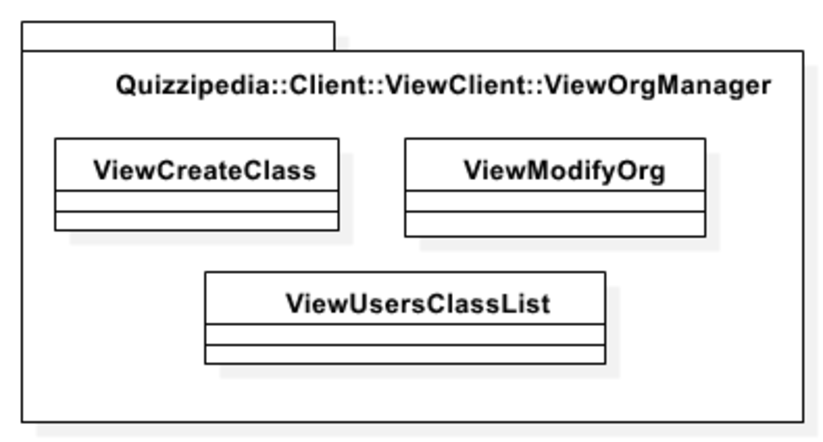
\includegraphics[width=\textwidth]{ImgST/quizzipedia-client-viewclient-vieworgmanager.pdf}}
\caption{Schema Componente Quizzipedia::Client::ViewClient::ViewOrgManager}
\end{figure}
\subsubsection{Classe ViewCreateClass}
Classe responsabile di creare la pagina da cui sarà possibile creare una nuova classe.
\begin{figure}[H]
\centering
\noindent\makebox[\textwidth]{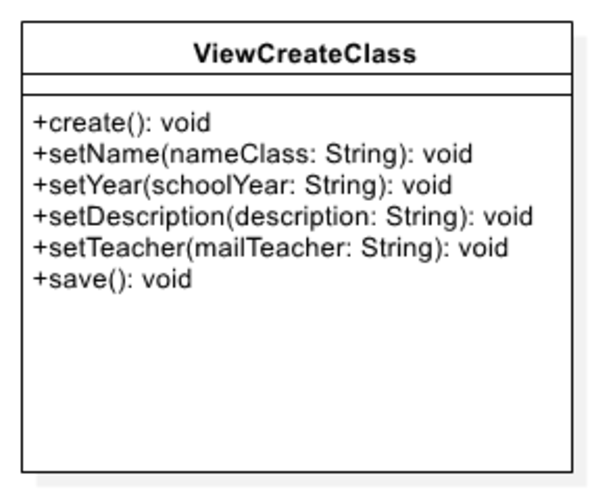
\includegraphics[width=\textwidth]{ImgST/quizzipedia-client-viewclient-vieworgmanager-viewcreateclass.pdf}}
\caption{Schema Classe Quizzipedia::Client::ViewClient::ViewOrgManager::ViewCreateClass}
\end{figure}
\subsubsection{Classe ViewModifyOrg}
Presenta all'utente la pagina da cui sarà possibile modificare le informazioni su una classe o su un ente esistente.
\begin{figure}[H]
\centering
\noindent\makebox[\textwidth]{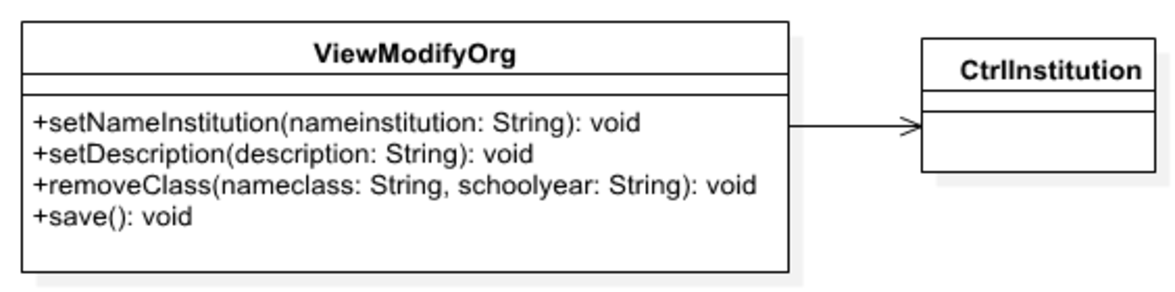
\includegraphics[width=\textwidth]{ImgST/quizzipedia-client-viewclient-vieworgmanager-viewmodifyorg.pdf}}
\caption{Schema Classe Quizzipedia::Client::ViewClient::ViewOrgManager::ViewModifyOrg}
\end{figure}
\subsubsection{Classe ViewUsersClassList}
La classe si occupa di presentare una lista degli utenti iscritti alla classe e altre informazioni aggiuntive.
\begin{figure}[H]
\centering
\noindent\makebox[\textwidth]{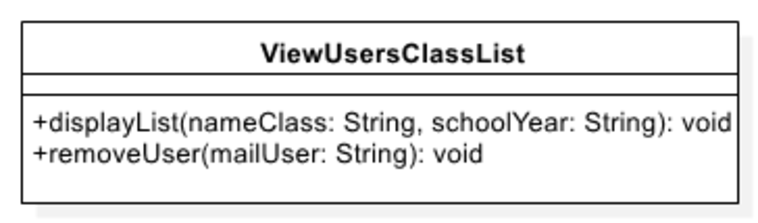
\includegraphics[width=\textwidth]{ImgST/quizzipedia-client-viewclient-vieworgmanager-viewusersclasslist.pdf}}
\caption{Schema Classe Quizzipedia::Client::ViewClient::ViewOrgManager::ViewUsersClassList}
\end{figure}
\subsection{Quizzipedia::Client::ViewClient::ViewQuestionManager}
Qui sono raccolte le classi responsabili della presentazione delle pagine da cui sarà possibile gestire le domande.
\begin{figure}[H]
\centering
\noindent\makebox[\textwidth]{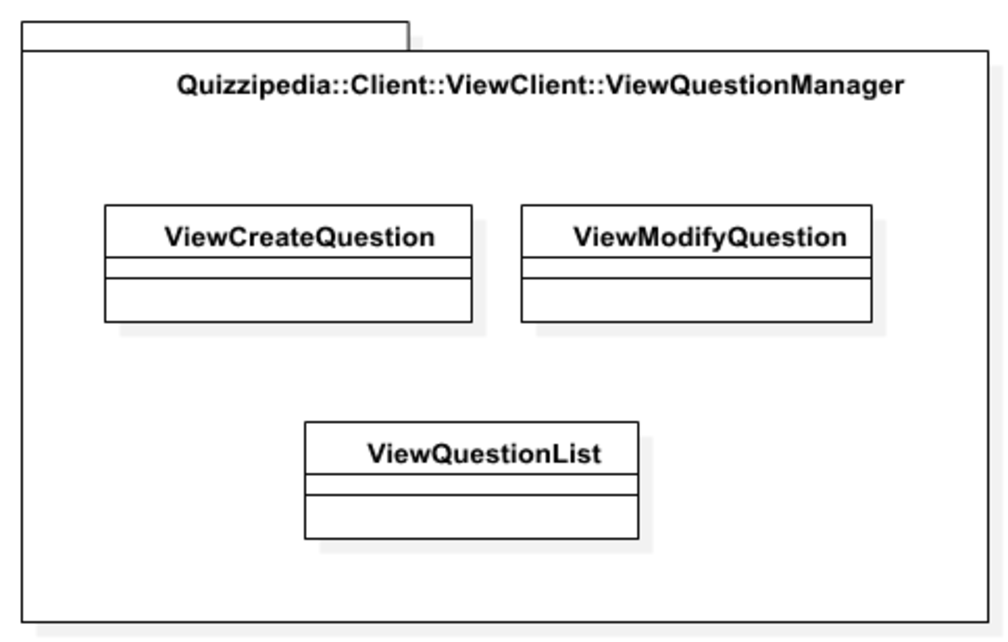
\includegraphics[width=\textwidth]{ImgST/quizzipedia-client-viewclient-viewquestionmanager.pdf}}
\caption{Schema Componente Quizzipedia::Client::ViewClient::ViewQuestionManager}
\end{figure}
\subsubsection{Classe ViewCreateQuestion}
Presenta la pagina da cui sarà possibile creare una nuova domanda.
\begin{figure}[H]
\centering
\noindent\makebox[\textwidth]{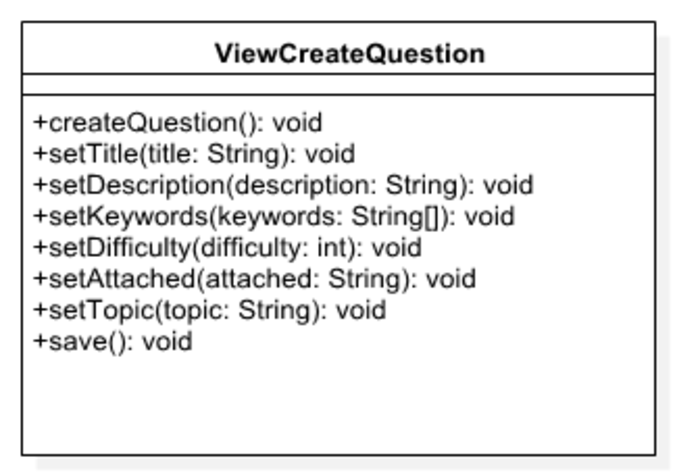
\includegraphics[width=\textwidth]{ImgST/quizzipedia-client-viewclient-viewquestionmanager-viewcreatequestion.pdf}}
\caption{Schema Classe Quizzipedia::Client::ViewClient::ViewQuestionManager::ViewCreateQuestion}
\end{figure}
\subsubsection{Classe ViewModifyQuestion}
Gestisce la visualizzazione della pagina da cui è possibile modificare una domanda esistente.
\begin{figure}[H]
\centering
\noindent\makebox[\textwidth]{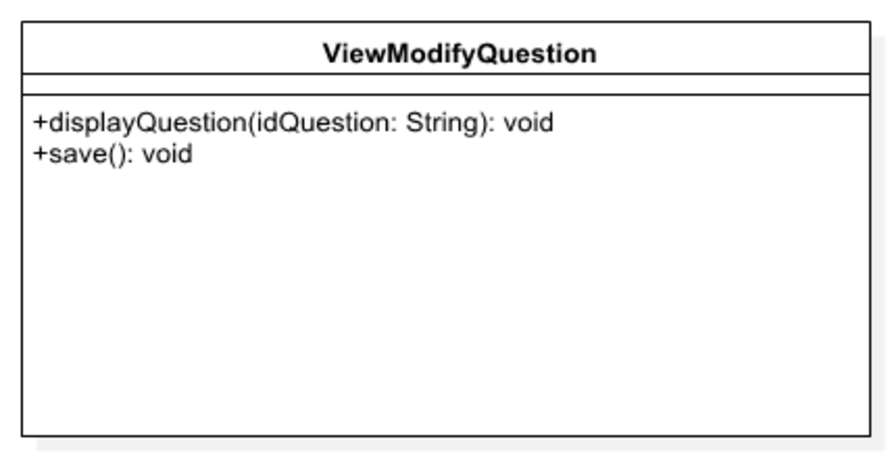
\includegraphics[width=\textwidth]{ImgST/quizzipedia-client-viewclient-viewquestionmanager-viewmodifyquestion.pdf}}
\caption{Schema Classe Quizzipedia::Client::ViewClient::ViewQuestionManager::ViewModifyQuestion}
\end{figure}
\subsubsection{Classe ViewQuestionList}
Presenta all'utente il pannello da cui sarà possibile visualizzare una lista di informazioni riassuntive sulle domande e compiere alcune operazioni su di esse.
\begin{figure}[H]
\centering
\noindent\makebox[\textwidth]{\includegraphics[width=\textwidth]{ImgST/quizzipedia-client-viewclient-viewquestionmanager-viewquestionlist.pdf}}
\caption{Schema Classe Quizzipedia::Client::ViewClient::ViewQuestionManager::ViewQuestionList}
\end{figure}
\subsection{Quizzipedia::Client::ViewClient::ViewQuizManager}
Qui sono raccolte le classi responsabili della presentazione delle pagine da cui sarà possibile gestire i quiz.
\begin{figure}[H]
\centering
\noindent\makebox[\textwidth]{\includegraphics[width=\textwidth]{ImgST/quizzipedia-client-viewclient-viewquizmanager.pdf}}
\caption{Schema Componente Quizzipedia::Client::ViewClient::ViewQuizManager}
\end{figure}
\subsubsection{Classe ViewCreateQuiz}
Presenta la pagina da cui sarà possibile creare un nuovo quiz.
\begin{figure}[H]
\centering
\noindent\makebox[\textwidth]{\includegraphics[width=\textwidth]{ImgST/quizzipedia-client-viewclient-viewquizmanager-viewcreatequiz.pdf}}
\caption{Schema Classe Quizzipedia::Client::ViewClient::ViewQuizManager::ViewCreateQuiz}
\end{figure}
\subsubsection{Classe ViewModifyQuiz}
Presenta all'utente una pagina da cui è possibile modificare un quiz esistente.
\begin{figure}[H]
\centering
\noindent\makebox[\textwidth]{\includegraphics[width=\textwidth]{ImgST/quizzipedia-client-viewclient-viewquizmanager-viewmodifyquiz.pdf}}
\caption{Schema Classe Quizzipedia::Client::ViewClient::ViewQuizManager::ViewModifyQuiz}
\end{figure}
\subsubsection{Classe ViewQuizList}
Carica una pagina contenente una lista con informazioni riassuntive sui quiz e un pannello da cui sarà possibile svolgere delle operazioni sugli stessi.
\begin{figure}[H]
\centering
\noindent\makebox[\textwidth]{\includegraphics[width=\textwidth]{ImgST/quizzipedia-client-viewclient-viewquizmanager-viewquizlist.pdf}}
\caption{Schema Classe Quizzipedia::Client::ViewClient::ViewQuizManager::ViewQuizList}
\end{figure}
\subsection{Quizzipedia::Client::ViewClient::ViewQuizSolver}
Il package raccoglie le classi necessarie alla visualizzazione delle pagine da cui sarà possibile svolgere quiz.
\begin{figure}[H]
\centering
\noindent\makebox[\textwidth]{\includegraphics[width=\textwidth]{ImgST/quizzipedia-client-viewclient-viewquizsolver.pdf}}
\caption{Schema Componente Quizzipedia::Client::ViewClient::ViewQuizSolver}
\end{figure}
\subsubsection{Componenti contenute}
\begin{itemize}
\item Quizzipedia::Client::ViewClient::ViewQuizSolver::ViewQuestionSolver
\end{itemize}
\subsubsection{Classe ViewResults}
La classe ha il compito di costruire la pagina da cui sarà possibile vedere l'esito di un quiz.
\begin{figure}[H]
\centering
\noindent\makebox[\textwidth]{\includegraphics[width=\textwidth]{ImgST/quizzipedia-client-viewclient-viewquizsolver-viewresults.pdf}}
\caption{Schema Classe Quizzipedia::Client::ViewClient::ViewQuizSolver::ViewResults}
\end{figure}
\subsection{Quizzipedia::Client::ViewClient::ViewQuizSolver::ViewQuestionSolver}
Il package raccoglie le classi necessarie alla visualizzazione delle pagine da cui sarà possibile rispondere alle singole domande.
\begin{figure}[H]
\centering
\noindent\makebox[\textwidth]{\includegraphics[width=\textwidth]{ImgST/quizzipedia-client-viewclient-viewquizsolver-viewquestionsolver.pdf}}
\caption{Schema Componente Quizzipedia::Client::ViewClient::ViewQuizSolver::ViewQuestionSolver}
\end{figure}
\subsubsection{Classe ViewCompletionQ}
Presenta all'utente la pagina da cui sarà possibile rispondere a una domanda a completamento.
\begin{figure}[H]
\centering
\noindent\makebox[\textwidth]{\includegraphics[width=\textwidth]{ImgST/quizzipedia-client-viewclient-viewquizsolver-viewquestionsolver-viewcompletionq.pdf}}
\caption{Schema Classe Quizzipedia::Client::ViewClient::ViewQuizSolver::ViewQuestionSolver::ViewCompletionQ}
\end{figure}
\subsubsection{Classe ViewMatchingQ}
Presenta all'utente la pagina da cui sarà possibile rispondere a una domanda a collegamenti.
\begin{figure}[H]
\centering
\noindent\makebox[\textwidth]{\includegraphics[width=\textwidth]{ImgST/quizzipedia-client-viewclient-viewquizsolver-viewquestionsolver-viewmatchingq.pdf}}
\caption{Schema Classe Quizzipedia::Client::ViewClient::ViewQuizSolver::ViewQuestionSolver::ViewMatchingQ}
\end{figure}
\subsubsection{Classe ViewMultipleChoiceQ}
Presenta all'utente la pagina da cui sarà possibile rispondere a una domanda a risposta multipla.
\begin{figure}[H]
\centering
\noindent\makebox[\textwidth]{\includegraphics[width=\textwidth]{ImgST/quizzipedia-client-viewclient-viewquizsolver-viewquestionsolver-viewmultiplechoiceq.pdf}}
\caption{Schema Classe Quizzipedia::Client::ViewClient::ViewQuizSolver::ViewQuestionSolver::ViewMultipleChoiceQ}
\end{figure}
\subsubsection{Classe ViewShortAnswerQ}
Presenta all'utente la pagina da cui sarà possibile rispondere a una domanda a risposta aperta.
\begin{figure}[H]
\centering
\noindent\makebox[\textwidth]{\includegraphics[width=\textwidth]{ImgST/quizzipedia-client-viewclient-viewquizsolver-viewquestionsolver-viewshortanswerq.pdf}}
\caption{Schema Classe Quizzipedia::Client::ViewClient::ViewQuizSolver::ViewQuestionSolver::ViewShortAnswerQ}
\end{figure}
\subsubsection{Classe ViewTrueFalseQ}
Presenta all'utente la pagina da cui sarà possibile rispondere a una domanda di tipo vero/falso.
\begin{figure}[H]
\centering
\noindent\makebox[\textwidth]{\includegraphics[width=\textwidth]{ImgST/quizzipedia-client-viewclient-viewquizsolver-viewquestionsolver-viewtruefalseq.pdf}}
\caption{Schema Classe Quizzipedia::Client::ViewClient::ViewQuizSolver::ViewQuestionSolver::ViewTrueFalseQ}
\end{figure}
\subsection{Quizzipedia::Client::ViewClient::ViewRequests}
Qui sono raccolte le pagine che permettono all'utente di gestire le richieste di ruolo e classe.
\begin{figure}[H]
\centering
\noindent\makebox[\textwidth]{\includegraphics[width=\textwidth]{ImgST/quizzipedia-client-viewclient-viewrequests.pdf}}
\caption{Schema Componente Quizzipedia::Client::ViewClient::ViewRequests}
\end{figure}
\subsubsection{Classe RequestClass}
Costruisce la pagina da cui l'utente potrà richiedere di entrare in una classe.
\begin{figure}[H]
\centering
\noindent\makebox[\textwidth]{\includegraphics[width=\textwidth]{ImgST/quizzipedia-client-viewclient-viewrequests-requestclass.pdf}}
\caption{Schema Classe Quizzipedia::Client::ViewClient::ViewRequests::RequestClass}
\end{figure}
\subsubsection{Classe RequestRole}
Costruisce la pagina da cui l'utente potrà richiedere un ruolo (studente o docente).
\begin{figure}[H]
\centering
\noindent\makebox[\textwidth]{\includegraphics[width=\textwidth]{ImgST/quizzipedia-client-viewclient-viewrequests-requestrole.pdf}}
\caption{Schema Classe Quizzipedia::Client::ViewClient::ViewRequests::RequestRole}
\end{figure}
\subsubsection{Classe ViewClassList}
Classe responsabile della visualizzazione del pannello da cui sarà possibile gestire le richieste di inserimento in una classe.
\begin{figure}[H]
\centering
\noindent\makebox[\textwidth]{\includegraphics[width=\textwidth]{ImgST/quizzipedia-client-viewclient-viewrequests-viewclasslist.pdf}}
\caption{Schema Classe Quizzipedia::Client::ViewClient::ViewRequests::ViewClassList}
\end{figure}
\subsubsection{Classe ViewRolesList}
Classe responsabile della visualizzazione del pannello da cui sarà possibile gestire le richieste di assegnazione di ruolo.
\begin{figure}[H]
\centering
\noindent\makebox[\textwidth]{\includegraphics[width=\textwidth]{ImgST/quizzipedia-client-viewclient-viewrequests-viewroleslist.pdf}}
\caption{Schema Classe Quizzipedia::Client::ViewClient::ViewRequests::ViewRolesList}
\end{figure}
\subsection{Quizzipedia::Client::ViewClient::ViewSearch}
Il package contiene le classi responsabili della creazione delle pagine da cui sarà possibile ricercare domande, quiz e classi .
\begin{figure}[H]
\centering
\noindent\makebox[\textwidth]{\includegraphics[width=\textwidth]{ImgST/quizzipedia-client-viewclient-viewsearch.pdf}}
\caption{Schema Componente Quizzipedia::Client::ViewClient::ViewSearch}
\end{figure}
\subsubsection{Classe ViewSearchClass}
La classe carica la pagina da cui sarà possibile ricercare classi all'interno di un ente.
\begin{figure}[H]
\centering
\noindent\makebox[\textwidth]{\includegraphics[width=\textwidth]{ImgST/quizzipedia-client-viewclient-viewsearch-viewsearchclass.pdf}}
\caption{Schema Classe Quizzipedia::Client::ViewClient::ViewSearch::ViewSearchClass}
\end{figure}
\subsubsection{Classe ViewSearchQuestion}
Classe che ha il compito di caricare la pagina da cui sarà possibile effettuare la ricerca di domande.
\begin{figure}[H]
\centering
\noindent\makebox[\textwidth]{\includegraphics[width=\textwidth]{ImgST/quizzipedia-client-viewclient-viewsearch-viewsearchquestion.pdf}}
\caption{Schema Classe Quizzipedia::Client::ViewClient::ViewSearch::ViewSearchQuestion}
\end{figure}
\subsubsection{Classe ViewSearchQuiz}
Raccoglie i metodi necessari alla creazione della pagina da cui sarà possibile cercare un quiz.
\begin{figure}[H]
\centering
\noindent\makebox[\textwidth]{\includegraphics[width=\textwidth]{ImgST/quizzipedia-client-viewclient-viewsearch-viewsearchquiz.pdf}}
\caption{Schema Classe Quizzipedia::Client::ViewClient::ViewSearch::ViewSearchQuiz}
\end{figure}
\subsection{Quizzipedia::Client::ViewClient::ViewStatistics}
Package che gestisce le pagine in cui verranno visualizzate le statistiche.
\begin{figure}[H]
\centering
\noindent\makebox[\textwidth]{\includegraphics[width=\textwidth]{ImgST/quizzipedia-client-viewclient-viewstatistics.pdf}}
\caption{Schema Componente Quizzipedia::Client::ViewClient::ViewStatistics}
\end{figure}
\subsubsection{Classe ViewClassStats}
Vengono rappresentate le statistiche relative a una singola classe in relazione a un particolare quiz.
\begin{figure}[H]
\centering
\noindent\makebox[\textwidth]{\includegraphics[width=\textwidth]{ImgST/quizzipedia-client-viewclient-viewstatistics-viewclassstats.pdf}}
\caption{Schema Classe Quizzipedia::Client::ViewClient::ViewStatistics::ViewClassStats}
\end{figure}
\subsubsection{Classe ViewQuestionStats}
Vengono rappresentate le statistiche generali relative alle domande.
\begin{figure}[H]
\centering
\noindent\makebox[\textwidth]{\includegraphics[width=\textwidth]{ImgST/quizzipedia-client-viewclient-viewstatistics-viewquestionstats.pdf}}
\caption{Schema Classe Quizzipedia::Client::ViewClient::ViewStatistics::ViewQuestionStats}
\end{figure}
\subsubsection{Classe ViewQuizStats}
Vengono rappresentate le statistiche generali riguardanti i quiz.
\begin{figure}[H]
\centering
\noindent\makebox[\textwidth]{\includegraphics[width=\textwidth]{ImgST/quizzipedia-client-viewclient-viewstatistics-viewquizstats.pdf}}
\caption{Schema Classe Quizzipedia::Client::ViewClient::ViewStatistics::ViewQuizStats}
\end{figure}
\subsection{Quizzipedia::Client::ViewClient::ViewTopicManager}
Qui sono raccolte le classi responsabili della presentazione delle pagine da cui sarà possibile gestire gli argomenti di domande e quiz.
\begin{figure}[H]
\centering
\noindent\makebox[\textwidth]{\includegraphics[width=\textwidth]{ImgST/quizzipedia-client-viewclient-viewtopicmanager.pdf}}
\caption{Schema Componente Quizzipedia::Client::ViewClient::ViewTopicManager}
\end{figure}
\subsubsection{Classe ViewCreateTopic}
La classe caricherà la pagina da cui sarà possibile creare un nuovo argomento.
\begin{figure}[H]
\centering
\noindent\makebox[\textwidth]{\includegraphics[width=\textwidth]{ImgST/quizzipedia-client-viewclient-viewtopicmanager-viewcreatetopic.pdf}}
\caption{Schema Classe Quizzipedia::Client::ViewClient::ViewTopicManager::ViewCreateTopic}
\end{figure}
\subsubsection{Classe ViewTopicList}
La classe è responsabile della creazione della pagina da cui sarà possibile vedere la lista degli argomenti disponibili.
\begin{figure}[H]
\centering
\noindent\makebox[\textwidth]{\includegraphics[width=\textwidth]{ImgST/quizzipedia-client-viewclient-viewtopicmanager-viewtopiclist.pdf}}
\caption{Schema Classe Quizzipedia::Client::ViewClient::ViewTopicManager::ViewTopicList}
\end{figure}
\subsection{Quizzipedia::Client::ViewClient::ViewUsers}
Raccoglie le classi necessarie a presentare all'utente le pagine da cui visualizzare le informazioni che lo riguardano e compiere le funzioni principali.
\begin{figure}[H]
\centering
\noindent\makebox[\textwidth]{\includegraphics[width=\textwidth]{ImgST/quizzipedia-client-viewclient-viewusers.pdf}}
\caption{Schema Componente Quizzipedia::Client::ViewClient::ViewUsers}
\end{figure}
\subsubsection{Classe Login}
Presenta la pagina necessaria per effettuare il login nel sistema.
\begin{figure}[H]
\centering
\noindent\makebox[\textwidth]{\includegraphics[width=\textwidth]{ImgST/quizzipedia-client-viewclient-viewusers-login.pdf}}
\caption{Schema Classe Quizzipedia::Client::ViewClient::ViewUsers::Login}
\end{figure}
\subsubsection{Classe Logout}
Presenta la pagina necessaria per effettuare il logout dal sistema.
\begin{figure}[H]
\centering
\noindent\makebox[\textwidth]{\includegraphics[width=\textwidth]{ImgST/quizzipedia-client-viewclient-viewusers-logout.pdf}}
\caption{Schema Classe Quizzipedia::Client::ViewClient::ViewUsers::Logout}
\end{figure}
\subsubsection{Classe Menu}
Presenta all'utente il menu da cui potrà svolgere le proprie funzioni principali.
\begin{figure}[H]
\centering
\noindent\makebox[\textwidth]{\includegraphics[width=\textwidth]{ImgST/quizzipedia-client-viewclient-viewusers-menu.pdf}}
\caption{Schema Classe Quizzipedia::Client::ViewClient::ViewUsers::Menu}
\end{figure}
\subsubsection{Classe PersonalData}
La classe presenta all'utente la pagina da cui prendere visione delle proprie informazioni personali.
\begin{figure}[H]
\centering
\noindent\makebox[\textwidth]{\includegraphics[width=\textwidth]{ImgST/quizzipedia-client-viewclient-viewusers-personaldata.pdf}}
\caption{Schema Classe Quizzipedia::Client::ViewClient::ViewUsers::PersonalData}
\end{figure}
\subsubsection{Classe RecoveryPw}
Da questa pagina sarà possibile inserire i dati per il recupero della password.
\begin{figure}[H]
\centering
\noindent\makebox[\textwidth]{\includegraphics[width=\textwidth]{ImgST/quizzipedia-client-viewclient-viewusers-recoverypw.pdf}}
\caption{Schema Classe Quizzipedia::Client::ViewClient::ViewUsers::RecoveryPw}
\end{figure}
\subsubsection{Classe Registration}
Presenta la pagina da cui effettuare la  registrazione al sistema.
\begin{figure}[H]
\centering
\noindent\makebox[\textwidth]{\includegraphics[width=\textwidth]{ImgST/quizzipedia-client-viewclient-viewusers-registration.pdf}}
\caption{Schema Classe Quizzipedia::Client::ViewClient::ViewUsers::Registration}
\end{figure}
\subsubsection{Classe ViewModifyUser}
Da qui, grazie ai metodi della classe, l'utente potrà modificare le proprie informazioni personali.
\begin{figure}[H]
\centering
\noindent\makebox[\textwidth]{\includegraphics[width=\textwidth]{ImgST/quizzipedia-client-viewclient-viewusers-viewmodifyuser.pdf}}
\caption{Schema Classe Quizzipedia::Client::ViewClient::ViewUsers::ViewModifyUser}
\end{figure}
\subsubsection{Classe ViewUsersList}
Presenta un pannello da cui è possibile visualizzare una lista di utenti e compiere operazioni su di loro.
\begin{figure}[H]
\centering
\noindent\makebox[\textwidth]{\includegraphics[width=\textwidth]{ImgST/quizzipedia-client-viewclient-viewusers-viewuserslist.pdf}}
\caption{Schema Classe Quizzipedia::Client::ViewClient::ViewUsers::ViewUsersList}
\end{figure}
\subsection{Quizzipedia::Client::ControllerClient}
Raccoglie le classi responsabili della comunicazione tra il model e la view.
\begin{figure}[H]
\centering
\noindent\makebox[\textwidth]{\includegraphics[width=\textwidth]{ImgST/quizzipedia-client-controllerclient.pdf}}
\caption{Schema Componente Quizzipedia::Client::ControllerClient}
\end{figure}
\subsubsection{Componenti contenute}
\begin{itemize}
\item Quizzipedia::Client::ControllerClient::CtrlOrganization
\item Quizzipedia::Client::ControllerClient::CtrlRequests
\item Quizzipedia::Client::ControllerClient::CtrlServices
\item Quizzipedia::Client::ControllerClient::CtrlStatistics
\item Quizzipedia::Client::ControllerClient::CtrlUsers
\end{itemize}
\subsection{Quizzipedia::Client::ControllerClient::CtrlOrganization}
Raccoglie le classi che si occupano delle comunicazioni necessarie per la creazione di enti e classi.
\begin{figure}[H]
\centering
\noindent\makebox[\textwidth]{\includegraphics[width=\textwidth]{ImgST/quizzipedia-client-controllerclient-ctrlorganization.pdf}}
\caption{Schema Componente Quizzipedia::Client::ControllerClient::CtrlOrganization}
\end{figure}
\subsubsection{Classe CtrlClass}
Vi sono presenti metodi necessari alla creazione delle classi.
\begin{figure}[H]
\centering
\noindent\makebox[\textwidth]{\includegraphics[width=\textwidth]{ImgST/quizzipedia-client-controllerclient-ctrlorganization-ctrlclass.pdf}}
\caption{Schema Classe Quizzipedia::Client::ControllerClient::CtrlOrganization::CtrlClass}
\end{figure}
\subsubsection{Classe CtrlInstitution}
Vi sono presenti metodi necessari alla creazione degli enti.
\begin{figure}[H]
\centering
\noindent\makebox[\textwidth]{\includegraphics[width=\textwidth]{ImgST/quizzipedia-client-controllerclient-ctrlorganization-ctrlinstitution.pdf}}
\caption{Schema Classe Quizzipedia::Client::ControllerClient::CtrlOrganization::CtrlInstitution}
\end{figure}
\subsection{Quizzipedia::Client::ControllerClient::CtrlRequests}
Questo package contiene classi necessarie alla gestione delle richieste di ruolo o classe.
\begin{figure}[H]
\centering
\noindent\makebox[\textwidth]{\includegraphics[width=\textwidth]{ImgST/quizzipedia-client-controllerclient-ctrlrequests.pdf}}
\caption{Schema Componente Quizzipedia::Client::ControllerClient::CtrlRequests}
\end{figure}
\subsubsection{Classe CtrlRequestClass}
Si occupa delle comunicazioni necessarie per la gestione delle richieste di inserimento in una classe.
\begin{figure}[H]
\centering
\noindent\makebox[\textwidth]{\includegraphics[width=\textwidth]{ImgST/quizzipedia-client-controllerclient-ctrlrequests-ctrlrequestclass.pdf}}
\caption{Schema Classe Quizzipedia::Client::ControllerClient::CtrlRequests::CtrlRequestClass}
\end{figure}
\subsubsection{Classe CtrlRequestRole}
Si occupa delle comunicazioni necessarie per la gestione delle richieste di ruolo.
\begin{figure}[H]
\centering
\noindent\makebox[\textwidth]{\includegraphics[width=\textwidth]{ImgST/quizzipedia-client-controllerclient-ctrlrequests-ctrlrequestrole.pdf}}
\caption{Schema Classe Quizzipedia::Client::ControllerClient::CtrlRequests::CtrlRequestRole}
\end{figure}
\subsection{Quizzipedia::Client::ControllerClient::CtrlServices}
Raccoglie gli elementi necessari alla creazione, svolgimento e ricerca di quiz e domande.
\begin{figure}[H]
\centering
\noindent\makebox[\textwidth]{\includegraphics[width=\textwidth]{ImgST/quizzipedia-client-controllerclient-ctrlservices.pdf}}
\caption{Schema Componente Quizzipedia::Client::ControllerClient::CtrlServices}
\end{figure}
\subsubsection{Classe CtrlQuestion}
Fornisce i metodi necessari per la comunicazione tra view e model durante la creazione, modifica e svolgimento di una domanda.
\begin{figure}[H]
\centering
\noindent\makebox[\textwidth]{\includegraphics[width=\textwidth]{ImgST/quizzipedia-client-controllerclient-ctrlservices-ctrlquestion.pdf}}
\caption{Schema Classe Quizzipedia::Client::ControllerClient::CtrlServices::CtrlQuestion}
\end{figure}
\subsubsection{Classe CtrlQuiz}
Raccoglie i metodi necessari nelle comunicazioni tra view e model richieste per la gestione e lo svolgimento dei quiz.
\begin{figure}[H]
\centering
\noindent\makebox[\textwidth]{\includegraphics[width=\textwidth]{ImgST/quizzipedia-client-controllerclient-ctrlservices-ctrlquiz.pdf}}
\caption{Schema Classe Quizzipedia::Client::ControllerClient::CtrlServices::CtrlQuiz}
\end{figure}
\subsubsection{Classe CtrlSearch}
La classe contiene i metodi necessari alla comunicazione tra model e view nell'effetuare la ricerca di quiz o domande.
\begin{figure}[H]
\centering
\noindent\makebox[\textwidth]{\includegraphics[width=\textwidth]{ImgST/quizzipedia-client-controllerclient-ctrlservices-ctrlsearch.pdf}}
\caption{Schema Classe Quizzipedia::Client::ControllerClient::CtrlServices::CtrlSearch}
\end{figure}
\subsubsection{Classe CtrlTopics}
Fornisce i metodi necessari alle comunicazioni richieste per la gestione degli argomenti.
\begin{figure}[H]
\centering
\noindent\makebox[\textwidth]{\includegraphics[width=\textwidth]{ImgST/quizzipedia-client-controllerclient-ctrlservices-ctrltopics.pdf}}
\caption{Schema Classe Quizzipedia::Client::ControllerClient::CtrlServices::CtrlTopics}
\end{figure}
\subsection{Quizzipedia::Client::ControllerClient::CtrlStatistics}
Raccoglie le classi necessarie a recuperare le statistiche da presentare all'utente.
\begin{figure}[H]
\centering
\noindent\makebox[\textwidth]{\includegraphics[width=\textwidth]{ImgST/quizzipedia-client-controllerclient-ctrlstatistics.pdf}}
\caption{Schema Componente Quizzipedia::Client::ControllerClient::CtrlStatistics}
\end{figure}
\subsubsection{Classe CtrlStats}
Classe necessaria al caricamento delle statistiche relative ai quiz, alle domande e alle classi.
\begin{figure}[H]
\centering
\noindent\makebox[\textwidth]{\includegraphics[width=\textwidth]{ImgST/quizzipedia-client-controllerclient-ctrlstatistics-ctrlstats.pdf}}
\caption{Schema Classe Quizzipedia::Client::ControllerClient::CtrlStatistics::CtrlStats}
\end{figure}
\subsection{Quizzipedia::Client::ControllerClient::CtrlUsers}
Il package raccoglie le classi che permettono la comunicazione per quanto riguarda funzioni e dati dell'utente.
\begin{figure}[H]
\centering
\noindent\makebox[\textwidth]{\includegraphics[width=\textwidth]{ImgST/quizzipedia-client-controllerclient-ctrlusers.pdf}}
\caption{Schema Componente Quizzipedia::Client::ControllerClient::CtrlUsers}
\end{figure}
\subsubsection{Classe CtrlData}
La classe raccoglie i metodi per gestire le informazioni personali di tutti gli utenti autenticati.
\begin{figure}[H]
\centering
\noindent\makebox[\textwidth]{\includegraphics[width=\textwidth]{ImgST/quizzipedia-client-controllerclient-ctrlusers-ctrldata.pdf}}
\caption{Schema Classe Quizzipedia::Client::ControllerClient::CtrlUsers::CtrlData}
\end{figure}
\subsubsection{Classe CtrlUserManager}
La classe permette agli utenti di gestire il proprio profilo personale.
\begin{figure}[H]
\centering
\noindent\makebox[\textwidth]{\includegraphics[width=\textwidth]{ImgST/quizzipedia-client-controllerclient-ctrlusers-ctrlusermanager.pdf}}
\caption{Schema Classe Quizzipedia::Client::ControllerClient::CtrlUsers::CtrlUserManager}
\end{figure}
\subsection{Quizzipedia::Server}
Racchiude tutte le componenti necessarie per il back-end del prodotto. Contiene anche le componenti che si occupano del QML.
\begin{figure}[H]
\centering
\noindent\makebox[\textwidth]{\includegraphics[width=\textwidth]{ImgST/quizzipedia-server.pdf}}
\caption{Schema Componente Quizzipedia::Server}
\end{figure}
\subsection{Quizzipedia::Server::ModelServer}
Rappresenta il modello dei dati che verranno utilizzati dal sistema lato server.
\begin{figure}[H]
\centering
\noindent\makebox[\textwidth]{\includegraphics[width=\textwidth]{ImgST/quizzipedia-server-modelserver.pdf}}
\caption{Schema Componente Quizzipedia::Server::ModelServer}
\end{figure}
\subsubsection{Componenti contenute}
\begin{itemize}
\item Quizzipedia::Server::ModelServer::Services
\end{itemize}
\subsection{Quizzipedia::Server::ModelServer::Services}
Il package racchiude i modelli necessari alla creazione di domande e quiz, i servizi principali offerti dal nostro prodotto.
\begin{figure}[H]
\centering
\noindent\makebox[\textwidth]{\includegraphics[width=\textwidth]{ImgST/quizzipedia-server-modelserver-services.pdf}}
\caption{Schema Componente Quizzipedia::Server::ModelServer::Services}
\end{figure}
\subsubsection{Componenti contenute}
\begin{itemize}
\item Quizzipedia::Server::ModelServer::Services::Questions
\end{itemize}
\subsubsection{Classe Info}
Riassume le informazioni principali su quiz e domande, necessarie per una presentazione sintetica e puntuale all'utente. È poi possibile risalire alla domanda o al quiz completi.
\begin{figure}[H]
\centering
\noindent\makebox[\textwidth]{\includegraphics[width=\textwidth]{ImgST/quizzipedia-server-modelserver-services-info.pdf}}
\caption{Schema Classe Quizzipedia::Server::ModelServer::Services::Info}
\end{figure}
\subsubsection{Classe Quiz}
Include la struttura del quiz.
\begin{figure}[H]
\centering
\noindent\makebox[\textwidth]{\includegraphics[width=\textwidth]{ImgST/quizzipedia-server-modelserver-services-quiz.pdf}}
\caption{Schema Classe Quizzipedia::Server::ModelServer::Services::Quiz}
\end{figure}
\subsubsection{Classe Topics}
Modella la struttura necessaria a memorizzare la lista di argomenti. A ogni domanda e a ogni quiz verranno poi associati i relativi argomenti.
\begin{figure}[H]
\centering
\noindent\makebox[\textwidth]{\includegraphics[width=\textwidth]{ImgST/quizzipedia-server-modelserver-services-topics.pdf}}
\caption{Schema Classe Quizzipedia::Server::ModelServer::Services::Topics}
\end{figure}
\subsection{Quizzipedia::Server::ModelServer::Services::Questions}
Descrive il modo in cui sono strutturati i vari tipi di domande che l'utente può incontrare durante la creazione o la compilazione di quiz.
\begin{figure}[H]
\centering
\noindent\makebox[\textwidth]{\includegraphics[width=\textwidth]{ImgST/quizzipedia-server-modelserver-services-questions.pdf}}
\caption{Schema Componente Quizzipedia::Server::ModelServer::Services::Questions}
\end{figure}
\subsubsection{Classe Cell}
La classe descrive ogni singola riga (quindi ogni opzione) della colonna della domanda a collegamento.
\begin{figure}[H]
\centering
\noindent\makebox[\textwidth]{\includegraphics[width=\textwidth]{ImgST/quizzipedia-server-modelserver-services-questions-cell.pdf}}
\caption{Schema Classe Quizzipedia::Server::ModelServer::Services::Questions::Cell}
\end{figure}
\subsubsection{Classe Column}
La classe descrive le colonne della domanda a collegamenti.
\begin{figure}[H]
\centering
\noindent\makebox[\textwidth]{\includegraphics[width=\textwidth]{ImgST/quizzipedia-server-modelserver-services-questions-column.pdf}}
\caption{Schema Classe Quizzipedia::Server::ModelServer::Services::Questions::Column}
\end{figure}
\subsubsection{Classe CompletationQ}
Descrive le domande a completamento. Il docente fornirà un testo incompleto e una lista di possibili completamenti; lo studente dovrà inserire le parole adeguate nella giusta posizione.
\begin{figure}[H]
\centering
\noindent\makebox[\textwidth]{\includegraphics[width=\textwidth]{ImgST/quizzipedia-server-modelserver-services-questions-completationq.pdf}}
\caption{Schema Classe Quizzipedia::Server::ModelServer::Services::Questions::CompletationQ}
\end{figure}
\subsubsection{Classe GenericQuestion}
Descrive le parti comuni a tutti i tipi di domanda presenti nel sistema.
\begin{figure}[H]
\centering
\noindent\makebox[\textwidth]{\includegraphics[width=\textwidth]{ImgST/quizzipedia-server-modelserver-services-questions-genericquestion.pdf}}
\caption{Schema Classe Quizzipedia::Server::ModelServer::Services::Questions::GenericQuestion}
\end{figure}
\subsubsection{Classe MatchingQ}
La struttura descrive le domande a collegamento. L'utente dovrà formare la risposa collegando entrate da un numero variabile di colonne.
\begin{figure}[H]
\centering
\noindent\makebox[\textwidth]{\includegraphics[width=\textwidth]{ImgST/quizzipedia-server-modelserver-services-questions-matchingq.pdf}}
\caption{Schema Classe Quizzipedia::Server::ModelServer::Services::Questions::MatchingQ}
\end{figure}
\subsubsection{Classe MultipleChoiceQ}
La struttura descrive le domande a scelta multipla; viene presentata una lista di opzioni tra cui scegliere quelle corrette.
\begin{figure}[H]
\centering
\noindent\makebox[\textwidth]{\includegraphics[width=\textwidth]{ImgST/quizzipedia-server-modelserver-services-questions-multiplechoiceq.pdf}}
\caption{Schema Classe Quizzipedia::Server::ModelServer::Services::Questions::MultipleChoiceQ}
\end{figure}
\subsubsection{Classe ShortAnswerQ}
La struttura descrive le domande aperte, ovvero quelle la cui risposta consiste in un termine o una frase specifici.
\begin{figure}[H]
\centering
\noindent\makebox[\textwidth]{\includegraphics[width=\textwidth]{ImgST/quizzipedia-server-modelserver-services-questions-shortanswerq.pdf}}
\caption{Schema Classe Quizzipedia::Server::ModelServer::Services::Questions::ShortAnswerQ}
\end{figure}
\subsubsection{Classe TrueFalseQ}
Viene descritta la struttura delle domande che prevedono di decidere la veridicità di un'affermazione.
\begin{figure}[H]
\centering
\noindent\makebox[\textwidth]{\includegraphics[width=\textwidth]{ImgST/quizzipedia-server-modelserver-services-questions-truefalseq.pdf}}
\caption{Schema Classe Quizzipedia::Server::ModelServer::Services::Questions::TrueFalseQ}
\end{figure}
\subsection{Quizzipedia::Server::ControllerServer}
Questo package contiene tutti i servizi che ricalcano il pattern architetturale DAO in modo da isolare l'accesso al database relazionale, controllando sempre che l'utente che genera una determinata richiesta al server sia abilitato per farla.
\begin{figure}[H]
\centering
\noindent\makebox[\textwidth]{\includegraphics[width=\textwidth]{ImgST/quizzipedia-server-controllerserver.pdf}}
\caption{Schema Componente Quizzipedia::Server::ControllerServer}
\end{figure}
\subsubsection{Componenti contenute}
\begin{itemize}
\item Quizzipedia::Server::ControllerServer::AuthenticationManager
\item Quizzipedia::Server::ControllerServer::ClassManager
\item Quizzipedia::Server::ControllerServer::CompanyManager
\item Quizzipedia::Server::ControllerServer::ProfileManager
\item Quizzipedia::Server::ControllerServer::QuestionsManager
\item Quizzipedia::Server::ControllerServer::QuizManager
\item Quizzipedia::Server::ControllerServer::RequestsManager
\item Quizzipedia::Server::ControllerServer::SearchManager
\item Quizzipedia::Server::ControllerServer::StatisticsManager
\item Quizzipedia::Server::ControllerServer::TopicManager
\end{itemize}
\subsection{Quizzipedia::Server::ControllerServer::AuthenticationManager}
Package che permette di gestire le funzioni basi per una corretta autenticazione al sistema.
\begin{figure}[H]
\centering
\noindent\makebox[\textwidth]{\includegraphics[width=\textwidth]{ImgST/quizzipedia-server-controllerserver-authenticationmanager.pdf}}
\caption{Schema Componente Quizzipedia::Server::ControllerServer::AuthenticationManager}
\end{figure}
\subsubsection{Classe LoggerIn}
Permette l'autenticazione nel sistema da parte di utenti preventivamente registrati.
\begin{figure}[H]
\centering
\noindent\makebox[\textwidth]{\includegraphics[width=\textwidth]{ImgST/quizzipedia-server-controllerserver-authenticationmanager-loggerin.pdf}}
\caption{Schema Classe Quizzipedia::Server::ControllerServer::AuthenticationManager::LoggerIn}
\end{figure}
\subsubsection{Classe LoggerOut}
Permette l'uscita dal sistema ad utenti autenticati.
\begin{figure}[H]
\centering
\noindent\makebox[\textwidth]{\includegraphics[width=\textwidth]{ImgST/quizzipedia-server-controllerserver-authenticationmanager-loggerout.pdf}}
\caption{Schema Classe Quizzipedia::Server::ControllerServer::AuthenticationManager::LoggerOut}
\end{figure}
\subsubsection{Classe PasswordRecover}
Permette il recupero della password da parte di un utente in caso di smarrimento o dimenticanza.
\begin{figure}[H]
\centering
\noindent\makebox[\textwidth]{\includegraphics[width=\textwidth]{ImgST/quizzipedia-server-controllerserver-authenticationmanager-passwordrecover.pdf}}
\caption{Schema Classe Quizzipedia::Server::ControllerServer::AuthenticationManager::PasswordRecover}
\end{figure}
\subsubsection{Classe Register}
Permette la registrazione di un utente nel sistema.
\begin{figure}[H]
\centering
\noindent\makebox[\textwidth]{\includegraphics[width=\textwidth]{ImgST/quizzipedia-server-controllerserver-authenticationmanager-register.pdf}}
\caption{Schema Classe Quizzipedia::Server::ControllerServer::AuthenticationManager::Register}
\end{figure}
\subsubsection{Classe SessionController}
Effettua il controllo sull'utente per verificare che egli sia in possesso dell'autorizzazione necessaria per compiere determinate richieste alla base di dati.
\begin{figure}[H]
\centering
\noindent\makebox[\textwidth]{\includegraphics[width=\textwidth]{ImgST/quizzipedia-server-controllerserver-authenticationmanager-sessioncontroller.pdf}}
\caption{Schema Classe Quizzipedia::Server::ControllerServer::AuthenticationManager::SessionController}
\end{figure}
\subsection{Quizzipedia::Server::ControllerServer::ClassManager}
Package che racchiude tutte le funzionalità adibite al salvataggio e alla visualizzazione delle informazioni riguardanti le classi di un ente.
\begin{figure}[H]
\centering
\noindent\makebox[\textwidth]{\includegraphics[width=\textwidth]{ImgST/quizzipedia-server-controllerserver-classmanager.pdf}}
\caption{Schema Componente Quizzipedia::Server::ControllerServer::ClassManager}
\end{figure}
\subsubsection{Classe ClassAdder}
Permette la creazione di una nuova classe.
\begin{figure}[H]
\centering
\noindent\makebox[\textwidth]{\includegraphics[width=\textwidth]{ImgST/quizzipedia-server-controllerserver-classmanager-classadder.pdf}}
\caption{Schema Classe Quizzipedia::Server::ControllerServer::ClassManager::ClassAdder}
\end{figure}
\subsubsection{Classe ClassDeleter}
Permette la rimozione delle classi dal sistema.
\begin{figure}[H]
\centering
\noindent\makebox[\textwidth]{\includegraphics[width=\textwidth]{ImgST/quizzipedia-server-controllerserver-classmanager-classdeleter.pdf}}
\caption{Schema Classe Quizzipedia::Server::ControllerServer::ClassManager::ClassDeleter}
\end{figure}
\subsubsection{Classe ClassUpdater}
Permette la modifica delle informazioni di base di una determinata classe.
\begin{figure}[H]
\centering
\noindent\makebox[\textwidth]{\includegraphics[width=\textwidth]{ImgST/quizzipedia-server-controllerserver-classmanager-classupdater.pdf}}
\caption{Schema Classe Quizzipedia::Server::ControllerServer::ClassManager::ClassUpdater}
\end{figure}
\subsubsection{Classe FromClassRemover}
Permette la rimozione di un utente da una determinata classe.
\begin{figure}[H]
\centering
\noindent\makebox[\textwidth]{\includegraphics[width=\textwidth]{ImgST/quizzipedia-server-controllerserver-classmanager-fromclassremover.pdf}}
\caption{Schema Classe Quizzipedia::Server::ControllerServer::ClassManager::FromClassRemover}
\end{figure}
\subsubsection{Classe InClassAdder}
Permette l'inserimento di un utente in una specifica classe.
\begin{figure}[H]
\centering
\noindent\makebox[\textwidth]{\includegraphics[width=\textwidth]{ImgST/quizzipedia-server-controllerserver-classmanager-inclassadder.pdf}}
\caption{Schema Classe Quizzipedia::Server::ControllerServer::ClassManager::InClassAdder}
\end{figure}
\subsubsection{Classe SessionController}
Effettua il controllo sull'utente per verificare che egli sia in possesso dell'autorizzazione necessaria per compiere determinate richieste alla base di dati.
\begin{figure}[H]
\centering
\noindent\makebox[\textwidth]{\includegraphics[width=\textwidth]{ImgST/quizzipedia-server-controllerserver-classmanager-sessioncontroller.pdf}}
\caption{Schema Classe Quizzipedia::Server::ControllerServer::ClassManager::SessionController}
\end{figure}
\subsubsection{Classe StudentsClassFetcher}
Recupera la lista degli studenti appartenenti ad una determinata classe.
\begin{figure}[H]
\centering
\noindent\makebox[\textwidth]{\includegraphics[width=\textwidth]{ImgST/quizzipedia-server-controllerserver-classmanager-studentsclassfetcher.pdf}}
\caption{Schema Classe Quizzipedia::Server::ControllerServer::ClassManager::StudentsClassFetcher}
\end{figure}
\subsubsection{Classe TeachersClassFetcher}
Recupera la lista degli insegnanti relativi ad una determinata classe.
\begin{figure}[H]
\centering
\noindent\makebox[\textwidth]{\includegraphics[width=\textwidth]{ImgST/quizzipedia-server-controllerserver-classmanager-teachersclassfetcher.pdf}}
\caption{Schema Classe Quizzipedia::Server::ControllerServer::ClassManager::TeachersClassFetcher}
\end{figure}
\subsection{Quizzipedia::Server::ControllerServer::CompanyManager}
Permette la gestione dell'ente da parte del responsabile.
\begin{figure}[H]
\centering
\noindent\makebox[\textwidth]{\includegraphics[width=\textwidth]{ImgST/quizzipedia-server-controllerserver-companymanager.pdf}}
\caption{Schema Componente Quizzipedia::Server::ControllerServer::CompanyManager}
\end{figure}
\subsubsection{Classe CompanyUpdater}
Permette la modifica dell'ente da parte del responsabile.
\begin{figure}[H]
\centering
\noindent\makebox[\textwidth]{\includegraphics[width=\textwidth]{ImgST/quizzipedia-server-controllerserver-companymanager-companyupdater.pdf}}
\caption{Schema Classe Quizzipedia::Server::ControllerServer::CompanyManager::CompanyUpdater}
\end{figure}
\subsubsection{Classe SessionController}
Effettua il controllo sull'utente per verificare che egli sia in possesso dell'autorizzazione necessaria per compiere determinate richieste alla base di dati.
\begin{figure}[H]
\centering
\noindent\makebox[\textwidth]{\includegraphics[width=\textwidth]{ImgST/quizzipedia-server-controllerserver-companymanager-sessioncontroller.pdf}}
\caption{Schema Classe Quizzipedia::Server::ControllerServer::CompanyManager::SessionController}
\end{figure}
\subsection{Quizzipedia::Server::ControllerServer::ProfileManager}
Package che racchiude tutte le funzionalità adibite al salvataggio e alla visualizzazione delle informazioni personali da parte di un utente autenticato.
\begin{figure}[H]
\centering
\noindent\makebox[\textwidth]{\includegraphics[width=\textwidth]{ImgST/quizzipedia-server-controllerserver-profilemanager.pdf}}
\caption{Schema Componente Quizzipedia::Server::ControllerServer::ProfileManager}
\end{figure}
\subsubsection{Classe AccountDeleter}
Permette la rimozione di un account dal sistema.
\begin{figure}[H]
\centering
\noindent\makebox[\textwidth]{\includegraphics[width=\textwidth]{ImgST/quizzipedia-server-controllerserver-profilemanager-accountdeleter.pdf}}
\caption{Schema Classe Quizzipedia::Server::ControllerServer::ProfileManager::AccountDeleter}
\end{figure}
\subsubsection{Classe PasswordSetter}
Permette ad un utente di impostare una nuova password relativa al proprio account.
\begin{figure}[H]
\centering
\noindent\makebox[\textwidth]{\includegraphics[width=\textwidth]{ImgST/quizzipedia-server-controllerserver-profilemanager-passwordsetter.pdf}}
\caption{Schema Classe Quizzipedia::Server::ControllerServer::ProfileManager::PasswordSetter}
\end{figure}
\subsubsection{Classe PersonalDataFetcher}
Ritorna tutte le informazioni personali riferite all'utente che ne effettua la richiesta.
\begin{figure}[H]
\centering
\noindent\makebox[\textwidth]{\includegraphics[width=\textwidth]{ImgST/quizzipedia-server-controllerserver-profilemanager-personaldatafetcher.pdf}}
\caption{Schema Classe Quizzipedia::Server::ControllerServer::ProfileManager::PersonalDataFetcher}
\end{figure}
\subsubsection{Classe PersonalDataSetter}
Permette ad un utente la modifica delle informazioni personali.
\begin{figure}[H]
\centering
\noindent\makebox[\textwidth]{\includegraphics[width=\textwidth]{ImgST/quizzipedia-server-controllerserver-profilemanager-personaldatasetter.pdf}}
\caption{Schema Classe Quizzipedia::Server::ControllerServer::ProfileManager::PersonalDataSetter}
\end{figure}
\subsubsection{Classe PersonalQuizFetcher}
Ritorna una lista contenente tutti i quiz che un utente autenticato ha svolto fino a quel momento.
\begin{figure}[H]
\centering
\noindent\makebox[\textwidth]{\includegraphics[width=\textwidth]{ImgST/quizzipedia-server-controllerserver-profilemanager-personalquizfetcher.pdf}}
\caption{Schema Classe Quizzipedia::Server::ControllerServer::ProfileManager::PersonalQuizFetcher}
\end{figure}
\subsubsection{Classe SessionController}
Effettua il controllo sull'utente per verificare che egli sia in possesso dell'autorizzazione necessaria per compiere determinate richieste alla base di dati.
\begin{figure}[H]
\centering
\noindent\makebox[\textwidth]{\includegraphics[width=\textwidth]{ImgST/quizzipedia-server-controllerserver-profilemanager-sessioncontroller.pdf}}
\caption{Schema Classe Quizzipedia::Server::ControllerServer::ProfileManager::SessionController}
\end{figure}
\subsection{Quizzipedia::Server::ControllerServer::QuestionsManager}
Pacchetto relativo alla gestione delle domande.
\begin{figure}[H]
\centering
\noindent\makebox[\textwidth]{\includegraphics[width=\textwidth]{ImgST/quizzipedia-server-controllerserver-questionsmanager.pdf}}
\caption{Schema Componente Quizzipedia::Server::ControllerServer::QuestionsManager}
\end{figure}
\subsubsection{Classe QuestionCreator}
Permette il salvataggio nella base di dati di una nuova domanda.
\begin{figure}[H]
\centering
\noindent\makebox[\textwidth]{\includegraphics[width=\textwidth]{ImgST/quizzipedia-server-controllerserver-questionsmanager-questioncreator.pdf}}
\caption{Schema Classe Quizzipedia::Server::ControllerServer::QuestionsManager::QuestionCreator}
\end{figure}
\subsubsection{Classe QuestionEraser}
Permette la cancellazione di una domanda dalla base di dati.
\begin{figure}[H]
\centering
\noindent\makebox[\textwidth]{\includegraphics[width=\textwidth]{ImgST/quizzipedia-server-controllerserver-questionsmanager-questioneraser.pdf}}
\caption{Schema Classe Quizzipedia::Server::ControllerServer::QuestionsManager::QuestionEraser}
\end{figure}
\subsubsection{Classe QuestionUpdater}
Permette la modifica di una domanda già esistente.
\begin{figure}[H]
\centering
\noindent\makebox[\textwidth]{\includegraphics[width=\textwidth]{ImgST/quizzipedia-server-controllerserver-questionsmanager-questionupdater.pdf}}
\caption{Schema Classe Quizzipedia::Server::ControllerServer::QuestionsManager::QuestionUpdater}
\end{figure}
\subsubsection{Classe SessionController}
Effettua il controllo sull'utente per verificare che egli sia in possesso dell'autorizzazione necessaria per compiere determinate richieste alla base di dati.
\begin{figure}[H]
\centering
\noindent\makebox[\textwidth]{\includegraphics[width=\textwidth]{ImgST/quizzipedia-server-controllerserver-questionsmanager-sessioncontroller.pdf}}
\caption{Schema Classe Quizzipedia::Server::ControllerServer::QuestionsManager::SessionController}
\end{figure}
\subsection{Quizzipedia::Server::ControllerServer::QuizManager}
Package che racchiude tutte le funzionalità adibite alla creazione, modifica e al recupero di quiz per lo svolgimento da parte di un utente.
\begin{figure}[H]
\centering
\noindent\makebox[\textwidth]{\includegraphics[width=\textwidth]{ImgST/quizzipedia-server-controllerserver-quizmanager.pdf}}
\caption{Schema Componente Quizzipedia::Server::ControllerServer::QuizManager}
\end{figure}
\subsubsection{Componenti contenute}
\begin{itemize}
\item Quizzipedia::Server::ControllerServer::QuizManager::QMLAgent
\end{itemize}
\subsubsection{Classe QuizCreator}
Permette il salvataggio nella base di dati di un nuovo quiz.
\begin{figure}[H]
\centering
\noindent\makebox[\textwidth]{\includegraphics[width=\textwidth]{ImgST/quizzipedia-server-controllerserver-quizmanager-quizcreator.pdf}}
\caption{Schema Classe Quizzipedia::Server::ControllerServer::QuizManager::QuizCreator}
\end{figure}
\subsubsection{Classe QuizEraser}
Permette la cancellazione di un quiz dalla base di dati.
\begin{figure}[H]
\centering
\noindent\makebox[\textwidth]{\includegraphics[width=\textwidth]{ImgST/quizzipedia-server-controllerserver-quizmanager-quizeraser.pdf}}
\caption{Schema Classe Quizzipedia::Server::ControllerServer::QuizManager::QuizEraser}
\end{figure}
\subsubsection{Classe QuizFetcher}
Ritorna un determinato quiz pronto per essere svolto da un utente .
\begin{figure}[H]
\centering
\noindent\makebox[\textwidth]{\includegraphics[width=\textwidth]{ImgST/quizzipedia-server-controllerserver-quizmanager-quizfetcher.pdf}}
\caption{Schema Classe Quizzipedia::Server::ControllerServer::QuizManager::QuizFetcher}
\end{figure}
\subsubsection{Classe QuizUpdater}
Permette la modifica di un quiz già presente nella base di dati.
\begin{figure}[H]
\centering
\noindent\makebox[\textwidth]{\includegraphics[width=\textwidth]{ImgST/quizzipedia-server-controllerserver-quizmanager-quizupdater.pdf}}
\caption{Schema Classe Quizzipedia::Server::ControllerServer::QuizManager::QuizUpdater}
\end{figure}
\subsubsection{Classe ResultsUpdater}
Aggiorna i risultati dei quiz ad ogni svolgimento degli stessi da parte dei un utente.
\begin{figure}[H]
\centering
\noindent\makebox[\textwidth]{\includegraphics[width=\textwidth]{ImgST/quizzipedia-server-controllerserver-quizmanager-resultsupdater.pdf}}
\caption{Schema Classe Quizzipedia::Server::ControllerServer::QuizManager::ResultsUpdater}
\end{figure}
\subsubsection{Classe SessionController}
Effettua il controllo sull'utente per verificare che egli sia in possesso dell'autorizzazione necessaria per compiere determinate richieste alla base di dati.
\begin{figure}[H]
\centering
\noindent\makebox[\textwidth]{\includegraphics[width=\textwidth]{ImgST/quizzipedia-server-controllerserver-quizmanager-sessioncontroller.pdf}}
\caption{Schema Classe Quizzipedia::Server::ControllerServer::QuizManager::SessionController}
\end{figure}
\subsubsection{Classe StatisticsUpdater}
Aggiorna le statistiche relative ad un quiz ogni volta che viene svolto da parte degli utenti.
\begin{figure}[H]
\centering
\noindent\makebox[\textwidth]{\includegraphics[width=\textwidth]{ImgST/quizzipedia-server-controllerserver-quizmanager-statisticsupdater.pdf}}
\caption{Schema Classe Quizzipedia::Server::ControllerServer::QuizManager::StatisticsUpdater}
\end{figure}
\subsection{Quizzipedia::Server::ControllerServer::QuizManager::QMLAgent}
Questo package racchiude i moduli necessari alla traduzione da QML ad un formato comprensibile dal sistema le informazioni estratte dal database per la generazione delle pagine HTML relative ad un quiz e viceversa.
\begin{figure}[H]
\centering
\noindent\makebox[\textwidth]{\includegraphics[width=\textwidth]{ImgST/quizzipedia-server-controllerserver-quizmanager-qmlagent.pdf}}
\caption{Schema Componente Quizzipedia::Server::ControllerServer::QuizManager::QMLAgent}
\end{figure}
\subsubsection{Classe QMLGenerator}
Permette la traduzione in formato QML di un quiz nel caso si voglia procedere al salvataggio dello stesso all'interno del database.
\begin{figure}[H]
\centering
\noindent\makebox[\textwidth]{\includegraphics[width=\textwidth]{ImgST/quizzipedia-server-controllerserver-quizmanager-qmlagent-qmlgenerator.pdf}}
\caption{Schema Classe Quizzipedia::Server::ControllerServer::QuizManager::QMLAgent::QMLGenerator}
\end{figure}
\subsubsection{Classe QMLParser}
Permette la traduzione di un quiz dal formato QML ad uno comprensibile dal sistema per la generazione delle relative pagine HTML.
\begin{figure}[H]
\centering
\noindent\makebox[\textwidth]{\includegraphics[width=\textwidth]{ImgST/quizzipedia-server-controllerserver-quizmanager-qmlagent-qmlparser.pdf}}
\caption{Schema Classe Quizzipedia::Server::ControllerServer::QuizManager::QMLAgent::QMLParser}
\end{figure}
\subsection{Quizzipedia::Server::ControllerServer::RequestsManager}
Package che si occupa di memorizzare richieste da parte degli utenti, mostrarle al responsabile e permettergli di accettarle o meno.
\begin{figure}[H]
\centering
\noindent\makebox[\textwidth]{\includegraphics[width=\textwidth]{ImgST/quizzipedia-server-controllerserver-requestsmanager.pdf}}
\caption{Schema Componente Quizzipedia::Server::ControllerServer::RequestsManager}
\end{figure}
\subsubsection{Classe ClassRequestsAdder}
Permette la memorizzazione delle richieste di creazione di una classe.
\begin{figure}[H]
\centering
\noindent\makebox[\textwidth]{\includegraphics[width=\textwidth]{ImgST/quizzipedia-server-controllerserver-requestsmanager-classrequestsadder.pdf}}
\caption{Schema Classe Quizzipedia::Server::ControllerServer::RequestsManager::ClassRequestsAdder}
\end{figure}
\subsubsection{Classe InsertClassRequestAdder}
Permette la memorizzazione nella base di dati di tutte le richieste da parte degli utenti di essere inseriti in una determinata classe.
\begin{figure}[H]
\centering
\noindent\makebox[\textwidth]{\includegraphics[width=\textwidth]{ImgST/quizzipedia-server-controllerserver-requestsmanager-insertclassrequestadder.pdf}}
\caption{Schema Classe Quizzipedia::Server::ControllerServer::RequestsManager::InsertClassRequestAdder}
\end{figure}
\subsubsection{Classe RequestsFetcher}
Permette la visualizzazione di tutte le richieste da parte degli utenti.
\begin{figure}[H]
\centering
\noindent\makebox[\textwidth]{\includegraphics[width=\textwidth]{ImgST/quizzipedia-server-controllerserver-requestsmanager-requestsfetcher.pdf}}
\caption{Schema Classe Quizzipedia::Server::ControllerServer::RequestsManager::RequestsFetcher}
\end{figure}
\subsubsection{Classe RoleAccepter}
Permette l'accettazione o la negazione dell'assegnazione di un ruolo ad un utente dopo che ne ha fatto richiesta.
\begin{figure}[H]
\centering
\noindent\makebox[\textwidth]{\includegraphics[width=\textwidth]{ImgST/quizzipedia-server-controllerserver-requestsmanager-roleaccepter.pdf}}
\caption{Schema Classe Quizzipedia::Server::ControllerServer::RequestsManager::RoleAccepter}
\end{figure}
\subsubsection{Classe RoleRequestsAdder}
Memorizza richieste da parte degli utenti di assumere un determinato ruolo all'interno del sistema.
\begin{figure}[H]
\centering
\noindent\makebox[\textwidth]{\includegraphics[width=\textwidth]{ImgST/quizzipedia-server-controllerserver-requestsmanager-rolerequestsadder.pdf}}
\caption{Schema Classe Quizzipedia::Server::ControllerServer::RequestsManager::RoleRequestsAdder}
\end{figure}
\subsubsection{Classe SessionController}
Effettua il controllo sull'utente per verificare che egli sia in possesso dell'autorizzazione necessaria per compiere determinate richieste alla base di dati.
\begin{figure}[H]
\centering
\noindent\makebox[\textwidth]{\includegraphics[width=\textwidth]{ImgST/quizzipedia-server-controllerserver-requestsmanager-sessioncontroller.pdf}}
\caption{Schema Classe Quizzipedia::Server::ControllerServer::RequestsManager::SessionController}
\end{figure}
\subsection{Quizzipedia::Server::ControllerServer::SearchManager}
Questo package permette di effettuare una ricerca nel database di quiz o domande richiesti dall'utente e ritornare una lista che corrisponde ai parametri desiderati.
\begin{figure}[H]
\centering
\noindent\makebox[\textwidth]{\includegraphics[width=\textwidth]{ImgST/quizzipedia-server-controllerserver-searchmanager.pdf}}
\caption{Schema Componente Quizzipedia::Server::ControllerServer::SearchManager}
\end{figure}
\subsubsection{Classe QuestionSearcher}
Ritorna una lista di domande che corrispondono ai parametri di ricerca impostati dall'utente.
\begin{figure}[H]
\centering
\noindent\makebox[\textwidth]{\includegraphics[width=\textwidth]{ImgST/quizzipedia-server-controllerserver-searchmanager-questionsearcher.pdf}}
\caption{Schema Classe Quizzipedia::Server::ControllerServer::SearchManager::QuestionSearcher}
\end{figure}
\subsubsection{Classe QuizSearcher}
Ritorna una lista di quiz che corrispondono ai parametri di ricerca impostati dall'utente.
\begin{figure}[H]
\centering
\noindent\makebox[\textwidth]{\includegraphics[width=\textwidth]{ImgST/quizzipedia-server-controllerserver-searchmanager-quizsearcher.pdf}}
\caption{Schema Classe Quizzipedia::Server::ControllerServer::SearchManager::QuizSearcher}
\end{figure}
\subsubsection{Classe SessionController}
Effettua il controllo sull'utente per verificare che egli sia in possesso dell'autorizzazione necessaria per compiere determinate richieste alla base di dati.
\begin{figure}[H]
\centering
\noindent\makebox[\textwidth]{\includegraphics[width=\textwidth]{ImgST/quizzipedia-server-controllerserver-searchmanager-sessioncontroller.pdf}}
\caption{Schema Classe Quizzipedia::Server::ControllerServer::SearchManager::SessionController}
\end{figure}
\subsection{Quizzipedia::Server::ControllerServer::StatisticsManager}
Questo package ha il compito di recuperare tutte le informazioni sottoforma di statistiche relative ad un quiz, una domanda in particolare o ad un utente.
\begin{figure}[H]
\centering
\noindent\makebox[\textwidth]{\includegraphics[width=\textwidth]{ImgST/quizzipedia-server-controllerserver-statisticsmanager.pdf}}
\caption{Schema Componente Quizzipedia::Server::ControllerServer::StatisticsManager}
\end{figure}
\subsubsection{Classe PersonalStatisticsFetcher}
Ritorna le statistiche personali.
\begin{figure}[H]
\centering
\noindent\makebox[\textwidth]{\includegraphics[width=\textwidth]{ImgST/quizzipedia-server-controllerserver-statisticsmanager-personalstatisticsfetcher.pdf}}
\caption{Schema Classe Quizzipedia::Server::ControllerServer::StatisticsManager::PersonalStatisticsFetcher}
\end{figure}
\subsubsection{Classe QuestionStatisticsFetcher}
Ritorna le statistiche riferite ad una domanda.
\begin{figure}[H]
\centering
\noindent\makebox[\textwidth]{\includegraphics[width=\textwidth]{ImgST/quizzipedia-server-controllerserver-statisticsmanager-questionstatisticsfetcher.pdf}}
\caption{Schema Classe Quizzipedia::Server::ControllerServer::StatisticsManager::QuestionStatisticsFetcher}
\end{figure}
\subsubsection{Classe QuizStatisticsFetcher}
Ritorna le statistiche riferite ad un quiz.
\begin{figure}[H]
\centering
\noindent\makebox[\textwidth]{\includegraphics[width=\textwidth]{ImgST/quizzipedia-server-controllerserver-statisticsmanager-quizstatisticsfetcher.pdf}}
\caption{Schema Classe Quizzipedia::Server::ControllerServer::StatisticsManager::QuizStatisticsFetcher}
\end{figure}
\subsubsection{Classe SessionController}
Effettua il controllo sull'utente per verificare che egli sia in possesso dell'autorizzazione necessaria per compiere determinate richieste alla base di dati.
\begin{figure}[H]
\centering
\noindent\makebox[\textwidth]{\includegraphics[width=\textwidth]{ImgST/quizzipedia-server-controllerserver-statisticsmanager-sessioncontroller.pdf}}
\caption{Schema Classe Quizzipedia::Server::ControllerServer::StatisticsManager::SessionController}
\end{figure}
\subsubsection{Classe StudentStatisticsFetcher}
Ritorna le statistiche riferite ad uno studente.
\begin{figure}[H]
\centering
\noindent\makebox[\textwidth]{\includegraphics[width=\textwidth]{ImgST/quizzipedia-server-controllerserver-statisticsmanager-studentstatisticsfetcher.pdf}}
\caption{Schema Classe Quizzipedia::Server::ControllerServer::StatisticsManager::StudentStatisticsFetcher}
\end{figure}
\subsubsection{Classe TeacherStatisticsFetcher}
Ritorna le statistiche riferite ad un docente.
\begin{figure}[H]
\centering
\noindent\makebox[\textwidth]{\includegraphics[width=\textwidth]{ImgST/quizzipedia-server-controllerserver-statisticsmanager-teacherstatisticsfetcher.pdf}}
\caption{Schema Classe Quizzipedia::Server::ControllerServer::StatisticsManager::TeacherStatisticsFetcher}
\end{figure}
\subsection{Quizzipedia::Server::ControllerServer::TopicManager}
Package che permette la creazione di un nuovo argomento o l'eliminazione di uno già esistente.
\begin{figure}[H]
\centering
\noindent\makebox[\textwidth]{\includegraphics[width=\textwidth]{ImgST/quizzipedia-server-controllerserver-topicmanager.pdf}}
\caption{Schema Componente Quizzipedia::Server::ControllerServer::TopicManager}
\end{figure}
\subsubsection{Classe SessionController}
Effettua il controllo sull'utente per verificare che egli sia in possesso dell'autorizzazione necessaria per compiere determinate richieste alla base di dati.
\begin{figure}[H]
\centering
\noindent\makebox[\textwidth]{\includegraphics[width=\textwidth]{ImgST/quizzipedia-server-controllerserver-topicmanager-sessioncontroller.pdf}}
\caption{Schema Classe Quizzipedia::Server::ControllerServer::TopicManager::SessionController}
\end{figure}
\subsubsection{Classe TopicCreator}
Permette la creazione di un nuovo argomento.
\begin{figure}[H]
\centering
\noindent\makebox[\textwidth]{\includegraphics[width=\textwidth]{ImgST/quizzipedia-server-controllerserver-topicmanager-topiccreator.pdf}}
\caption{Schema Classe Quizzipedia::Server::ControllerServer::TopicManager::TopicCreator}
\end{figure}
\subsubsection{Classe TopicEraser}
Permette l'eliminazione di un argomento.
\begin{figure}[H]
\centering
\noindent\makebox[\textwidth]{\includegraphics[width=\textwidth]{ImgST/quizzipedia-server-controllerserver-topicmanager-topiceraser.pdf}}
\caption{Schema Classe Quizzipedia::Server::ControllerServer::TopicManager::TopicEraser}
\end{figure}
\subsection{Quizzipedia::Server::RoutingManager}
Questo pachetto costituisce lo strato superiore a ControllerServer e contiene tutte le API necessarie per comunicare con il client tramite socket; esso ha il compito di indirizzare le richieste ai vari services in base alla richiesta da parte dell'utente.
\begin{figure}[H]
\centering
\noindent\makebox[\textwidth]{\includegraphics[width=\textwidth]{ImgST/quizzipedia-server-routingmanager.pdf}}
\caption{Schema Componente Quizzipedia::Server::RoutingManager}
\end{figure}
\subsubsection{Classe AuthenticationRouter}
Invocato dal client per interagire con AuthenticationManager.
\begin{figure}[H]
\centering
\noindent\makebox[\textwidth]{\includegraphics[width=\textwidth]{ImgST/quizzipedia-server-routingmanager-authenticationrouter.pdf}}
\caption{Schema Classe Quizzipedia::Server::RoutingManager::AuthenticationRouter}
\end{figure}
\subsubsection{Classe ClassRouter}
Invocato dal client per interagire con ClassManager.
\begin{figure}[H]
\centering
\noindent\makebox[\textwidth]{\includegraphics[width=\textwidth]{ImgST/quizzipedia-server-routingmanager-classrouter.pdf}}
\caption{Schema Classe Quizzipedia::Server::RoutingManager::ClassRouter}
\end{figure}
\subsubsection{Classe ProfileRouter}
Invocato dal client per interagire con ProfileManager.
\begin{figure}[H]
\centering
\noindent\makebox[\textwidth]{\includegraphics[width=\textwidth]{ImgST/quizzipedia-server-routingmanager-profilerouter.pdf}}
\caption{Schema Classe Quizzipedia::Server::RoutingManager::ProfileRouter}
\end{figure}
\subsubsection{Classe QuestionRouter}
Invocato dal client per interagire con QuestionsManager.
\begin{figure}[H]
\centering
\noindent\makebox[\textwidth]{\includegraphics[width=\textwidth]{ImgST/quizzipedia-server-routingmanager-questionrouter.pdf}}
\caption{Schema Classe Quizzipedia::Server::RoutingManager::QuestionRouter}
\end{figure}
\subsubsection{Classe QuizRouter}
Invocato dal client per interagire con QuizManager.
\begin{figure}[H]
\centering
\noindent\makebox[\textwidth]{\includegraphics[width=\textwidth]{ImgST/quizzipedia-server-routingmanager-quizrouter.pdf}}
\caption{Schema Classe Quizzipedia::Server::RoutingManager::QuizRouter}
\end{figure}
\subsubsection{Classe RequestsRouter}
Invocato dal client per interagire con RequestsManager.
\begin{figure}[H]
\centering
\noindent\makebox[\textwidth]{\includegraphics[width=\textwidth]{ImgST/quizzipedia-server-routingmanager-requestsrouter.pdf}}
\caption{Schema Classe Quizzipedia::Server::RoutingManager::RequestsRouter}
\end{figure}
\subsubsection{Classe SearchRouter}
Invocato dal client per interagire con SearchManager.
\begin{figure}[H]
\centering
\noindent\makebox[\textwidth]{\includegraphics[width=\textwidth]{ImgST/quizzipedia-server-routingmanager-searchrouter.pdf}}
\caption{Schema Classe Quizzipedia::Server::RoutingManager::SearchRouter}
\end{figure}
\subsubsection{Classe StatisticsRouter}
Invocato dal client per interagire con StatisticsManager.
\begin{figure}[H]
\centering
\noindent\makebox[\textwidth]{\includegraphics[width=\textwidth]{ImgST/quizzipedia-server-routingmanager-statisticsrouter.pdf}}
\caption{Schema Classe Quizzipedia::Server::RoutingManager::StatisticsRouter}
\end{figure}
\subsubsection{Classe TopicRouter}
Invocato dal client per interagire con TopicManager.
\begin{figure}[H]
\centering
\noindent\makebox[\textwidth]{\includegraphics[width=\textwidth]{ImgST/quizzipedia-server-routingmanager-topicrouter.pdf}}
\caption{Schema Classe Quizzipedia::Server::RoutingManager::TopicRouter}
\end{figure}
